\documentclass[]{elsarticle} %review=doublespace preprint=single 5p=2 column
%%% Begin My package additions %%%%%%%%%%%%%%%%%%%
\usepackage[hyphens]{url}

  \journal{Social Science \& Medicine} % Sets Journal name


\usepackage{lineno} % add

\usepackage{graphicx}
%%%%%%%%%%%%%%%% end my additions to header

\usepackage[T1]{fontenc}
\usepackage{lmodern}
\usepackage{amssymb,amsmath}
\usepackage{ifxetex,ifluatex}
\usepackage{fixltx2e} % provides \textsubscript
% use upquote if available, for straight quotes in verbatim environments
\IfFileExists{upquote.sty}{\usepackage{upquote}}{}
\ifnum 0\ifxetex 1\fi\ifluatex 1\fi=0 % if pdftex
  \usepackage[utf8]{inputenc}
\else % if luatex or xelatex
  \usepackage{fontspec}
  \ifxetex
    \usepackage{xltxtra,xunicode}
  \fi
  \defaultfontfeatures{Mapping=tex-text,Scale=MatchLowercase}
  \newcommand{\euro}{€}
\fi
% use microtype if available
\IfFileExists{microtype.sty}{\usepackage{microtype}}{}
\bibliographystyle{elsarticle-harv}
\ifxetex
  \usepackage[setpagesize=false, % page size defined by xetex
              unicode=false, % unicode breaks when used with xetex
              xetex]{hyperref}
\else
  \usepackage[unicode=true]{hyperref}
\fi
\hypersetup{breaklinks=true,
            bookmarks=true,
            pdfauthor={},
            pdftitle={How is active school travel framed in Ontario, Canada?},
            colorlinks=false,
            urlcolor=blue,
            linkcolor=magenta,
            pdfborder={0 0 0}}
\urlstyle{same}  % don't use monospace font for urls

\setcounter{secnumdepth}{0}
% Pandoc toggle for numbering sections (defaults to be off)
\setcounter{secnumdepth}{0}


% tightlist command for lists without linebreak
\providecommand{\tightlist}{%
  \setlength{\itemsep}{0pt}\setlength{\parskip}{0pt}}


% Pandoc citation processing
\newlength{\cslhangindent}
\setlength{\cslhangindent}{1.5em}
\newlength{\csllabelwidth}
\setlength{\csllabelwidth}{3em}
\newlength{\cslentryspacingunit} % times entry-spacing
\setlength{\cslentryspacingunit}{\parskip}
% for Pandoc 2.8 to 2.10.1
\newenvironment{cslreferences}%
  {}%
  {\par}
% For Pandoc 2.11+
\newenvironment{CSLReferences}[2] % #1 hanging-ident, #2 entry spacing
 {% don't indent paragraphs
  \setlength{\parindent}{0pt}
  % turn on hanging indent if param 1 is 1
  \ifodd #1
  \let\oldpar\par
  \def\par{\hangindent=\cslhangindent\oldpar}
  \fi
  % set entry spacing
  \setlength{\parskip}{#2\cslentryspacingunit}
 }%
 {}
\usepackage{calc}
\newcommand{\CSLBlock}[1]{#1\hfill\break}
\newcommand{\CSLLeftMargin}[1]{\parbox[t]{\csllabelwidth}{#1}}
\newcommand{\CSLRightInline}[1]{\parbox[t]{\linewidth - \csllabelwidth}{#1}\break}
\newcommand{\CSLIndent}[1]{\hspace{\cslhangindent}#1}

\usepackage{booktabs}
\usepackage{longtable}
\usepackage{array}
\usepackage{multirow}
\usepackage{wrapfig}
\usepackage{float}
\usepackage{colortbl}
\usepackage{pdflscape}
\usepackage{tabu}
\usepackage{threeparttable}
\usepackage{threeparttablex}
\usepackage[normalem]{ulem}
\usepackage{makecell}
\usepackage{xcolor}



\begin{document}


\begin{frontmatter}

  \title{How is active school travel framed in Ontario, Canada?}
    \author[Some Department]{Author 1\corref{1}}
   \ead{author1@example.com} 
    \author[Some Department]{Author 2}
   \ead{author2@example.com} 
    \author[Another University]{Author 3\corref{2}}
   \ead{author3@example.com} 
    \author[Some Institute]{Author 4\corref{2}}
   \ead{author4@example.com} 
    \author[Some University]{Author 5}
   \ead{author5@example.com} 
    \author[Some Department]{Author 6}
   \ead{author6@example.com} 
      \address[Some Department]{Department, Street, City, Province,
Postal Code}
    \address[Another University]{Department, Street, City, Province,
Postal Code}
    \address[Some Institute]{Street, City, Province, Postal Code}
    \address[Some University]{Department, Street, City, Province, Postal
Code}
      \cortext[1]{Corresponding Author}
    \cortext[2]{Equal contribution}
  
  \begin{abstract}
  Active school travel (AST) has been increasingly encouraged by various
  stakeholders in Ontario, Canada through efforts such as school travel
  planning. Education strategies like workshops or resources that
  promote AST are commonly implemented. The framing of AST through such
  strategies may influence how walking and bicycling to school are
  perceived by parents. It may also draw attention to AST as an issue
  affecting children's health which could motivate behaviour change. We
  used natural language processing, including topic modelling, to
  examine how AST is framed in publicly available documents from Ontario
  stakeholders involved in school travel planning. We then compared the
  findings from these documents to a selection of studies on AST and
  explored similarities between the two. We found that AST is framed in
  two ways: i) as a health and environmental issue; and ii) as an
  accessible and feasible transport option for children and parents. The
  frames encourage children and parents to adopt AST given its health
  and environmental benefits by providing resources to support behaviour
  change. The benefits of AST and strategies to support AST that are
  communicated by stakeholders are consistent with the evidence from
  academic research. While these frames present AST in a positive light,
  they may not encourage parents to view current household travel
  behaviours as unhealthy for their children or their community.
  Stakeholders promoting AST in Ontario should further problematize the
  decline of AST and challenge the norm of driving children to school.

  Keywords: active school travel, school travel planning; natural
  language processing; framing analysis; education strategies
  \end{abstract}
  
 \end{frontmatter}

\newpage

\hypertarget{introduction}{%
\section{1. Introduction}\label{introduction}}

Rates of walking and bicycling to school, commonly known as active
school travel (AST), have been declining in Canada and the United States
for decades (Rothman et al., 2018). However, the appetite for AST may be
high in many Canadian communities. For instance, in a study conducted in
Toronto, Ontario, 40\% of children who were driven to school stated they
would like to travel by bicycle instead (Larouche et al., 2016). The
study also reported that less than 3\% of respondents actually cycled,
despite the vast majority having access to a bicycle and living within a
short and bikeable distance to school. Another study based in London,
Ontario, reported similar findings with respect to children's preference
for active travel (Larsen et al., 2012). From a public health
perspective, increasing the use of active modes to school represents a
major opportunity to improve children's health and wellbeing.

The Government of Ontario, in Canada, has striven to promote this trend,
and created a fund in 2017 to support communities across the province to
develop AST initiatives. Green Communities Canada runs the program,
called \emph{Ontario Active School Travel} (G. C. Canada, 2020). As of
December 2021, OAST has awarded over CAD 2 million and provided
resources to over 25 projects across Ontario. Many communities
implemented school travel planning (STP), along with encouraging
activities like walking school buses and developed resources for schools
and parents, among other actions (see Canada, 2021). In this context,
STP is a popular ``school-specific'' intervention led by a facilitator
who brings together a committee of stakeholders from diverse sectors
including education, planning, transportation, and public health to
develop action plans (Buliung et al., 2011; Mammen et al., 2014a). The
five-step process involves identifying barriers to AST based on the
local context and implementing approaches or activities that make AST
safer and more convenient: 1) setup of the program; 2) data collection
and problem identification; 3) action planning; 4) implementation; 5)
monitoring and evaluation (Buliung et al., 2011; Lang et al., 2011).

How AST is framed by STP stakeholders to a target audience, like parents
or the general public, may raise awareness of the issue and influence
how walking and bicycling to school are perceived. Gamson and Modigliani
(1987) define a frame as a ``central organizing idea or story line that
provides meaning'' to a particular phenomenon. A frame can enable
individuals ``to locate, perceive, identify, and label'' information
pertaining to various dimensions of an issue (Goffman, 1974). Therefore,
stakeholders involved in STP efforts can play a role in shaping public
perception about AST in such a way that it attracts greater attention
and is recognized as a ``problem'' that needs to be addressed through
behaviour change or new policies.

After significant investment of human and financial resources to boost
rates of AST in Ontario over the past few years, we ask this central
question: How is AST framed to the public? The following questions are
subsidiary and help us address this main question: What benefits of AST
are communicated to the public? What solutions are proposed to increase
rates of AST?

In this paper, we use natural language processing to examine how three
STP stakeholder groups in Ontario (municipalities, school boards, and
transportation consortia) frame the issue of AST. We assembled a corpus
of texts from public sources that present information for the general
public or parents who are interested in AST. We examine word frequency,
bigrams, and concordances in these selected documents, and also identify
key topics presented by each stakeholder group. We then compare the
findings from these documents to a selection of studies on AST and
explore the extent to which there is concordance between the literature
on AST and materials shared with the public.

\hypertarget{literature-review}{%
\section{2. Literature Review}\label{literature-review}}

\hypertarget{benefits-of-active-school-travel}{%
\subsection{2.1. Benefits of active school
travel}\label{benefits-of-active-school-travel}}

There is value in communicating the benefits of AST to the public in
order to convey the importance of this issue. The desire to increase AST
in Canada is certainly warranted - there is compelling evidence of the
physical and mental health benefits that children who actively commute
to school attain. Faulkner et al. (2009) concluded from their systematic
review that children who travel on foot or by bicycle to school
generally have higher levels of physical activity than their peers who
are driven to school. However, Schoeppe et al. (2015) reported no
association between AST and physical activity in their cross-sectional
study. This relationship could be dose-dependent, meaning that children
would have to travel longer distances to accumulate physical activity. A
walking distance of 1000-1600 metres to school has been found to
contribute to overall levels of physical activity for boys (Faulkner et
al., 2013). The daily routine of travelling to school can be a good
opportunity for children to regularly build physical activity into their
schedule (Mitra, 2013). Research has also shown that using active modes
to school contributes to improve cardiovascular fitness (Børrestad et
al., 2012).

More recently, the literature has explored the link between transport
and children's wellbeing (Waygood et al., 2020), with relevant
applications to the study of travel satisfaction (van den Berg et al.,
2020; Westman et al., 2017b). Being driven to school reduces community
interactions for children, which may negatively impact their social
wellbeing (Waygood and Friman, 2015). In contrast, walking and bicycling
give children opportunities to socialize with friends or siblings
(Michail et al., 2021) and increase positive emotions that contribute to
wellbeing (Ramanathan et al., 2014). This is something that children
seem to value (Zwerts et al., 2010) and that tracks with findings among
university students (Páez and Whalen, 2010). More generally, social
connections through travel appear to be important for wellbeing.
Furthermore, AST can provide opportunities for children to engage with
natural environments (Fusco et al., 2012; Romero, 2015).

\hypertarget{factors-that-influence-active-school-travel-and-mode-choice}{%
\subsection{2.2. Factors that influence active school travel and mode
choice}\label{factors-that-influence-active-school-travel-and-mode-choice}}

Factors that influence AST have been presented and organized using a
socio-ecological model (SEM) (Mitra, 2013) or systems model (Badland et
al., 2016) whereby children's travel behaviour is understood within the
context of household, social, neighbourhood, and policy environments.
The SEM comes from the field of public health and is a useful framework
for understanding complex health behaviours, such as walking and
bicycling habits, This model helps to identify multiple determinants
that need to be addressed by interventions to facilitate behaviour
change. The consensus in the literature is that interventions should
target multiple levels in order to increase levels of healthy and
physically active modes of travel to school (Mitra, 2013). Rather than
describing an extensive list of factors that influence AST and mode
choice in Canada (e.g., Mammen et al., 2012; Mitra, 2013; Rothman et
al., 2018; Wilson et al., 2018), we discuss a few potentially modifiable
determinants that may be targeted for change through STP.

At the individual level, age is often positively associated with AST
(Mammen et al., 2012; Stark et al., 2018; Wilson et al., 2018). There is
evidence that gender is a determinant of AST, and that boys are more
likely to travel using active modes than girls, although this is not a
strong or consistent finding (Rothman et al., 2018; Schoeppe et al.,
2015). Children's mode choice to school is strongly influenced by their
parents' travel behaviours and the complexity of their household's
travel needs (Buliung et al., 2021), as well as daily parental support
(Mah et al., 2017). This indicates that shifting parental perceptions
and habits is important. Convenience and inclement weather have been
cited by parents as barriers to AST (Buliung et al., 2011). Parental
perceptions of the built or school environment (De Meester et al., 2014;
Panter et al., 2010) and their children's skills (Faulkner et al., 2010;
Mammen et al., 2012) also influence mode choice to school.

Distance between home and school is most negatively associated with AST
(Ikeda et al., 2018; Mammen et al., 2012; Pont et al., 2009; Rothman et
al., 2018) with less AST reported among children who have to travel
farther to school - low density suburban development tends to increase
the need for movement, and the reliance on motorized modes (Farber and
Páez, 2011). Many studies have also found that the quality of the built
environment along the route to school and around the school site (Ikeda
et al., 2018; Rothman et al., 2021) and provision of active travel
infrastructure (Chen et al., 2018; Pont et al., 2009) facilitate AST.
Canadian youth report that they feel most safe bicycling on streets in
their neighbourhood or that have low volumes of traffic (T. A. of
Canada, 2020). Finally, concerns about traffic and strangers have been
reported by parents who drive their children to school (Mammen et al.,
2012), which highlights that the volume and speed of cars can be a
concern or deterrent for AST.

\hypertarget{school-travel-planning-in-canada}{%
\subsection{2.3. School travel planning in
Canada}\label{school-travel-planning-in-canada}}

School travel planning (STP) has been implemented in Canada since at
least the late 2000s. Within the STP process, facilitators generally
establish multi-sector committees which intervene at the participating
school through a range of activities related to the 4E's consisting of
\emph{education} strategies, \emph{encouragement} through in-person
events or programs, \emph{engineering} improvements to or around the
school site, and \emph{enforcement} of traffic speeds around schools
(Lang et al., 2011; Mammen et al., 2014b). The first large-scale
evaluation of STP as an intervention in Canada took place at twelve
schools across the country, including four in Ontario, using parental
surveys to measure changes in travel behaviour and perceptions (Buliung
et al., 2011). Following the intervention, active travel rates increased
across all schools and 14\% of parents reported a perceived reduction in
traffic outside the school (Buliung et al., 2011). Assessments of the
efficacy of STP (Buttazzoni et al., 2019; Mammen et al., 2014b) indicate
that it has the potential to encourage behaviour change and adoption of
AST. STP facilitators have recommended that additional time and
resources are needed to improve the efficacy of STP (Mammen et al.,
2015), which highlights that long-term and sustained efforts driven at
the policy level are required to address declining rates of AST.

How AST is framed seems particularly important to shift parental
attitudes and perceptions, given their reported influence on children's
travel mode to school. STP activities heavily focus on education or
encouragement (Buliung et al., 2011; Buttazzoni et al., 2018; Mammen et
al., 2014b), but parents may not always be receptive to the goals of STP
and may be resistant to behaviour change (Buttazzoni et al., 2018).
Parents have been found to express different understandings, language,
and perceptions than planners of how the built environment can influence
school travel (Buliung et al., 2021). This is also true when it comes to
other factors like convenience of different modes to school (Lang et
al., 2011). STP stakeholders must pay special attention to parents'
understanding of the decline of AST as a problem, which may affect their
receptivity to proposed solutions.

The ``central organizing idea or story line'' of AST, to apply the
definition of framing from Gamson and Modigliani (1987), could also
affect broader support in the community. Municipal representatives are
perceived to be instrumental but the involvement of other stakeholder
groups (e.g., busing consortia representatives and local residents) can
be lacking (Buttazzoni et al., 2018). In Ontario, it is reasonable to
say that AST has become a policy issue on the education and public
health agendas, supported, albeit in a modest way, by financial
contributions from the provincial government\footnote{To put the CAD 2
  million invested by the province in the Ontario Active School Travel
  program in perspective, a city such as Hamilton budgeted in excess of
  CAD 91 million on road maintenance and construction in 2016 alone;
  see:
  https://www.hamilton.ca/budget-finance/city-budgets/2016-tax-and-rate-budgets}.
Still, the support from a range of municipal representatives (see
Buttazzoni et al., 2018; Mammen et al., 2015) demonstrates that the AST
issue is on the political agenda. However, it is unknown to what degree
the general public (i.e., local residents) has been exposed to messaging
about AST.

The success of STP interventions would likely depend on parental
judgments of factors that are related to school travel, as well as
support from key policy makers. For example, parents have been found to
view mixed land use as conducive for driving, despite transport planners
viewing neighbourhoods with mixed uses as key for encouraging more
active travel (Buliung et al., 2021). Therefore, stakeholders involved
in STP must make conscious choices about the proposed solutions and
potential benefits of AST that are communicated to parents and the
general public to convey its importance as a policy issue and to
facilitate adoption of AST. Publicly available content about AST needs
to effectively engage multiple audiences on this policy issue, including
parents, children, politicians, and school representatives. This
information should reflect current knowledge from research on school
travel, plus content specific to local factors that influence AST, so
that the challenges of AST are adequately defined and the opportunities
or solutions to address the problems are clear.

\hypertarget{framing-analysis}{%
\subsection{2.4. Framing Analysis}\label{framing-analysis}}

Issues that pertain to public health or wellbeing are often presented to
the public through particular frames to influence perceptions or
behaviours. As previously mentioned, a frame is a ``central organizing
idea or story line that provides meaning'' to a public issue or
phenomenon (Gamson and Modigliani, 1987). Scholars in the field of
political communications have proposed that communicators, such as the
media or institutions, construct the narrative of a frame for policy
positions or public issues in order to activate or restrict a particular
response in the intended audience (Pan and Kosicki, 1993). Organized
groups of stakeholders can employ similar methods to attract attention
to particular issues. Framing can be used to position existing solutions
as suitable to address particular issues (Mah et al., 2014), which may
prevent the public from being aware of other policy approaches that
challenge the status quo. The way policy issues are framed is ultimately
important to understand because it plays a role in either altering or
preserving the existing social perceptions. Finally, the ideas that are
communicated by a particular frame can be either positive or negative
(Waygood and Avineri, 2018). There is evidence that negative framing may
be more effective at motivating individuals to change transport modes to
reduce CO2 emissions (Waygood and Avineri, 2018).

Framing of issues is an important step in developing health policy. An
obvious example over the past decade is the framing of climate change as
a public health issue (e.g., Depoux et al., 2017; Maibach et al., 2010;
Weathers and Kendall, 2016) to increase public engagement and awareness
of the issue. This framing has slowly advanced this issue on public
policy agendas as public attention puts pressure on the policy stream to
adopt frameworks for action. For example, transport planners use
different frames to guide the extent to which transport policies can be
adapted to address climate change. In a recent paper (Reynard et al.,
2021), framing analysis was applied to review the representation of
issues such as mobility and social exclusion in municipal policies from
four western Canadian cities under the current circumstances of climate
change. The authors found four primary frames: ``The Growing City,''
``If You Build It, They Will Come,'' ``Better City for All,'' and a
``the Resilient City'' (Reynard et al., 2021). Each frame presented the
nature, opportunities, and challenges of climate change in different
ways which set the stage for the types of mitigation and adaptation
strategies that cities were proposing to address this issue.

In a similar way, we hypothesize that STP stakeholder groups in Ontario
have framed AST in particular ways to engage multiple audiences on this
policy issue including parents, local residents, school representatives,
and municipal representatives. These groups are likely identifying
points of intervention and potential opportunities to build support for
and encourage AST.

\hypertarget{data}{%
\section{3. Data}\label{data}}

\hypertarget{data-retrieval}{%
\subsection{3.1. Data retrieval}\label{data-retrieval}}

\hypertarget{policy-documents}{%
\subsubsection{3.1.1. Policy documents}\label{policy-documents}}

We assembled a collection of publicly available documents that were
sourced online from the main stakeholder groups involved in STP
initiatives in Ontario: i) school boards (public or Catholic and
English-speaking only); ii) municipal governments; and iii)
transportation consortia. The latter are a unique group of entities
sanctioned by Ontario's Ministry of Education in Ontario 2006. Each
consortium involves a collaboration between municipal regions and school
boards; the consortium's objective is to deliver more efficient and
timely transportation services to schools in each region. Non-profit
organizations, police services, and advocacy groups are other
stakeholders who often play a role in supporting AST and/or STP, but
this study does not include any documents from these groups because they
are not consistently participating in all initiatives across Ontario.

The search was guided first by a list of all English public and Catholic
school boards across Ontario. The websites of each school board were
manually searched for pages related to school transport or travel. Any
pages relevant to these topics were manually downloaded. Next, we
collected documents by searching municipal government and transportation
consortia websites. These were identified based on geographic area
(i.e., the municipalities and/or transportation consortia that are in
the same geographic area of each school board). Webpages related to
active transport or school travel were manually downloaded.

Webpages from STP stakeholder groups were included in our analysis if
they were easy to find. This primary criterion was important since our
analysis pertains to how such issues are framed to the general public.
Thus, we included only webpages that were readily accessible, which we
defined as requiring no more than 4 separate links from the initial
Google search.

The initial corpus of documents from STP stakeholder groups included 69
relevant webpages (i.e., one page or more). We refer to these as policy
documents throughout the paper. It is important to note that school
boards, municipalities, and transportation consortia may or may not
publish information about their involvement in AST and STP efforts on
their respective websites or in policy documents. Search results are
summarized in Table \ref{tab:policy-documents}.

\begin{table}

\caption{\label{tab:policy-documents}\label{tab:search-results}Search results from the main STP stakeholder groups.}
\centering
\begin{tabular}[t]{>{}l|l|>{}l}
\toprule
Stakeholder & Total & Retrieved\\
\midrule
\cellcolor{gray!6}{\textbf{School boards}} & \cellcolor{gray!6}{62} & \cellcolor{gray!6}{32}\\
\textbf{Municipalities} & 62 & 28\\
\cellcolor{gray!6}{\textbf{Transportation consortia}} & \cellcolor{gray!6}{39} & \cellcolor{gray!6}{9}\\
\bottomrule
\end{tabular}
\end{table}

\hypertarget{academic-papers}{%
\subsubsection{3.1.2. Academic papers}\label{academic-papers}}

We conducted a search on Web of Science for scholarly papers on the
topic of travel to school. We limited our search to the fields of public
health, transportation, planning, urban studies, and geography. This
initial corpus was curated by the authors to ensure that all documents
were relevant; for example, some hits in our search were not full papers
but conference reports, or they dealt with travel to school only
peripherally. After this step, we assembled a collection of 227 journal
articles for analysis.

\hypertarget{data-cleaning}{%
\subsection{3.2. Data cleaning}\label{data-cleaning}}

A multi-step process was conducted to ensure that the analysis captured
as much text as possible from both the policy documents (n = 64) and
academic papers (n = 227). To begin, the webpages, which were manually
downloaded in portable document format (PDF), were trimmed so that pages
that only consisted of tables, figures, or references were removed. Many
academic papers were in a two-column format, which is not ideal for
conversion to \texttt{txt}. Two-column PDF documents were processed to
extract the text in the correct sequence. Four academic papers did not
join sufficiently and were taken out of the corpus due to the
substantial time required to manually correct their inconsistencies.

Next, we converted the trimmed PDF documents into \texttt{txt} files so
that they could be imported for analysis in \texttt{R}. The next phase
was to manually remove any remaining tables, figures, references,
headers/footings, and captions that could not be trimmed. Manual
corrections were also required for certain pages in academic papers that
remained in two-column format after the conversion process. This
typically occurred on pages that had a table or figure that disrupted
the text. Finally, we reviewed all of the documents to remove
hyphenation by line breaks and to keep hyphenated words together on the
same line. Any ligatures (e.g., combinations of characters or letters
that were not properly detected during the conversion process) were
fixed.

We also manually removed any extraneous material that did not pertain to
AST specifically. For the academic papers, this included footnotes,
references, acknowledgments, and conflict of interest statements. For
the policy+practice documents, it included phone numbers, inserted links
to other webpages, personal names, and content not specific to AST. In
the final step, we removed all blank spaces, punctuation,
capitalization, and numbers. English stop words, which are common words
such as \emph{and} or \emph{the} as identified in a predetermined list
by Feinerer and Hornik (2020) and other frequent terms in the documents
like ``school'' and specific location names, were removed from the
corpora.

\hypertarget{methods}{%
\section{4. Methods}\label{methods}}

\hypertarget{process-of-framing-analysis}{%
\subsection{4.1. Process of Framing
Analysis}\label{process-of-framing-analysis}}

We use topic modelling in \texttt{R} to conduct the framing analysis.
Topic modelling is a machine learning technique used to analyze text to
identify the language and concepts being communicated. This method is
practical for researchers working with large amounts of text because it
replaces the manual coding of topics that would normally take place to
analyze or summarize textual data (Jacobi et al., 2016). In the data
pre-processing phase, we tokenize the text in the documents and create a
document-term matrix so that it is in the correct format for analysis.
We primarily use the following packages: \texttt{tidytext} (Robinson and
Silge, 2021), \texttt{topicmodels} (Grün and Hornik, 2021),
\texttt{word2vec} (Wijffels, 2021), and \texttt{wordcloud} (Fellows,
2018) to examine text in the documents that were sourced for this
project. These packages have functions for determining the frequency of
specific words in each document or relationships (e.g., pairs of
adjacent terms called bigrams) and correlations between words. Topic
modelling is a popular method for analyzing text from social media
platforms (Albalawi et al., 2020) and news articles (Jacobi et al.,
2016). We estimate latent Dirichlet allocation (LDA) models to classify
both the STP and academic documents according to the topics that are
contained within them. This method ``treats each document as a mixture
of topics, and each topic as a mixture of words'' (Silge and Robinson,
2022). The model's output is ``a set of topics consisting of clusters of
words that co-occur in these documents according to certain patterns''
(Jacobi et al., 2016). Researchers must then interpret the identified
topics, as done after other methods of manual coding. We also compare
the topics between the policy documents and the academic papers to
interpret what is being communicated by STP stakeholders. We describe in
more detail the functions and code in \texttt{R} that we used.

\hypertarget{reproducibility}{%
\subsection{4.3. Reproducibility}\label{reproducibility}}

This paper is an example of open and reproducible research that uses
only open software. Following best practices in spatial data science
(Brunsdon and Comber, 2020), the code and data needed to reproduce our
research or conduct a similar analysis for other regions are available
for download upon request.

\hypertarget{results}{%
\section{5. Results}\label{results}}

\hypertarget{word-and-document-frequency}{%
\subsection{5.1. Word and document
frequency}\label{word-and-document-frequency}}

We analyzed word and document frequency for each corpus of text. Table
\ref{tab:word-table} shows the most frequent terms found in the
municipal, transportation consortia, school board, and academic
documents. Policy documents and academic papers reference \emph{active},
\emph{travel}, \emph{walking}, \emph{biking} or \emph{cycling}, and
\emph{students} more than other terms. Each corpus also has
\emph{safety} and \emph{traffic} as common words which suggests that
these are common concerns for parents. The word \emph{physical} is
present in each corpus, but it's not clear what this refers to (e.g,
\emph{physical activity}, \emph{physical health}, or the \emph{physical
environment}). Furthermore, documents from STP stakeholder groups
discuss \emph{resources}, \emph{information}, and \emph{services} about
school travel. Unlike the academic papers, policy documents include the
words \emph{route} or \emph{routes} as frequent terms. This could
indicate the presence of ``safe routes to school'' in the policy corpus,
as well as the role of STP stakeholder groups in identifying safe routes
to school to share with parents or families. In the section below, the
context in which these terms are used is explored further.

The academic corpus differs from the policy documents in that
\emph{parents} and \emph{distance} are the second and third most common
terms. In addition, \emph{time}, \emph{factors}, \emph{environment}, and
\emph{age} are also identified in the academic papers. The prevalence of
these terms is consistent with an academic focus on exploring the
variables that influence mode choice. These words are absent from the
list of common words in policy documents. Table \ref{tab:word-table}
indicates that the academic corpus discusses a broader range of
determinants of AST than the policy documents. The number of references
for each term in the academic papers is also substantially higher due to
the inclusion of more documents.

\begin{table}

\caption{\label{tab:word-table}\label{tab:word-table}Top 25 terms identified in each corpus. Document frequencies are also indicated.}
\centering
\resizebox{\linewidth}{!}{
\begin{tabular}[t]{lcclcclcclcc}
\toprule
\multicolumn{3}{c}{Municipalities} & \multicolumn{3}{c}{School Boards} & \multicolumn{3}{c}{Transportation Consortia} & \multicolumn{3}{c}{Academic Papers} \\
\cmidrule(l{3pt}r{3pt}){1-3} \cmidrule(l{3pt}r{3pt}){4-6} \cmidrule(l{3pt}r{3pt}){7-9} \cmidrule(l{3pt}r{3pt}){10-12}
Term & Count (n) & Documents (n) & Term & Count (n) & Documents (n) & Term & Count (n) & Documents (n) & Term & Count (n) & Documents (n)\\
\midrule
\cellcolor{gray!6}{active} & \cellcolor{gray!6}{248} & \cellcolor{gray!6}{26} & \cellcolor{gray!6}{active} & \cellcolor{gray!6}{124} & \cellcolor{gray!6}{13} & \cellcolor{gray!6}{active} & \cellcolor{gray!6}{67} & \cellcolor{gray!6}{7} & \cellcolor{gray!6}{walking} & \cellcolor{gray!6}{5059} & \cellcolor{gray!6}{220}\\
travel & 126 & 20 & bus & 120 & 20 & walking & 55 & 8 & parents & 3927 & 209\\
\cellcolor{gray!6}{walking} & \cellcolor{gray!6}{90} & \cellcolor{gray!6}{25} & \cellcolor{gray!6}{travel} & \cellcolor{gray!6}{103} & \cellcolor{gray!6}{11} & \cellcolor{gray!6}{walk} & \cellcolor{gray!6}{49} & \cellcolor{gray!6}{8} & \cellcolor{gray!6}{distance} & \cellcolor{gray!6}{3252} & \cellcolor{gray!6}{203}\\
bike & 87 & 15 & information & 65 & 21 & travel & 41 & 8 & students & 2956 & 171\\
\cellcolor{gray!6}{cycling} & \cellcolor{gray!6}{78} & \cellcolor{gray!6}{22} & \cellcolor{gray!6}{walking} & \cellcolor{gray!6}{57} & \cellcolor{gray!6}{17} & \cellcolor{gray!6}{students} & \cellcolor{gray!6}{39} & \cellcolor{gray!6}{9} & \cellcolor{gray!6}{cycling} & \cellcolor{gray!6}{2739} & \cellcolor{gray!6}{170}\\
\addlinespace
safety & 71 & 21 & walk & 53 & 13 & safety & 32 & 6 & environment & 2585 & 200\\
\cellcolor{gray!6}{health} & \cellcolor{gray!6}{65} & \cellcolor{gray!6}{21} & \cellcolor{gray!6}{weather} & \cellcolor{gray!6}{40} & \cellcolor{gray!6}{11} & \cellcolor{gray!6}{help} & \cellcolor{gray!6}{29} & \cellcolor{gray!6}{9} & \cellcolor{gray!6}{traffic} & \cellcolor{gray!6}{2334} & \cellcolor{gray!6}{206}\\
physical & 63 & 18 & safety & 40 & 19 & schools & 25 & 9 & choice & 2295 & 167\\
\cellcolor{gray!6}{traffic} & \cellcolor{gray!6}{59} & \cellcolor{gray!6}{20} & \cellcolor{gray!6}{safe} & \cellcolor{gray!6}{39} & \cellcolor{gray!6}{19} & \cellcolor{gray!6}{children} & \cellcolor{gray!6}{25} & \cellcolor{gray!6}{6} & \cellcolor{gray!6}{activity} & \cellcolor{gray!6}{2265} & \cellcolor{gray!6}{207}\\
road & 56 & 13 & services & 37 & 17 & community & 24 & 7 & physical & 2238 & 213\\
\addlinespace
\cellcolor{gray!6}{activity} & \cellcolor{gray!6}{55} & \cellcolor{gray!6}{14} & \cellcolor{gray!6}{planning} & \cellcolor{gray!6}{37} & \cellcolor{gray!6}{7} & \cellcolor{gray!6}{bus} & \cellcolor{gray!6}{18} & \cellcolor{gray!6}{4} & \cellcolor{gray!6}{trips} & \cellcolor{gray!6}{2164} & \cellcolor{gray!6}{168}\\
schools & 52 & 14 & parents & 32 & 17 & route & 17 & 5 & car & 2140 & 193\\
\cellcolor{gray!6}{children} & \cellcolor{gray!6}{47} & \cellcolor{gray!6}{15} & \cellcolor{gray!6}{sustainable} & \cellcolor{gray!6}{31} & \cellcolor{gray!6}{8} & \cellcolor{gray!6}{zone} & \cellcolor{gray!6}{16} & \cellcolor{gray!6}{6} & \cellcolor{gray!6}{safety} & \cellcolor{gray!6}{2111} & \cellcolor{gray!6}{202}\\
plan & 45 & 16 & children & 31 & 14 & resources & 16 & 6 & time & 2091 & 216\\
\cellcolor{gray!6}{students} & \cellcolor{gray!6}{44} & \cellcolor{gray!6}{14} & \cellcolor{gray!6}{child} & \cellcolor{gray!6}{31} & \cellcolor{gray!6}{12} & \cellcolor{gray!6}{day} & \cellcolor{gray!6}{16} & \cellcolor{gray!6}{4} & \cellcolor{gray!6}{factors} & \cellcolor{gray!6}{2083} & \cellcolor{gray!6}{214}\\
\addlinespace
walk & 43 & 18 & day & 29 & 13 & safe & 15 & 5 & child & 2060 & 185\\
\cellcolor{gray!6}{public} & \cellcolor{gray!6}{39} & \cellcolor{gray!6}{15} & \cellcolor{gray!6}{routes} & \cellcolor{gray!6}{28} & \cellcolor{gray!6}{14} & \cellcolor{gray!6}{planning} & \cellcolor{gray!6}{15} & \cellcolor{gray!6}{4} & \cellcolor{gray!6}{walk} & \cellcolor{gray!6}{1985} & \cellcolor{gray!6}{198}\\
community & 37 & 19 & physical & 28 & 11 & physical & 15 & 7 & public & 1973 & 206\\
\cellcolor{gray!6}{safe} & \cellcolor{gray!6}{34} & \cellcolor{gray!6}{16} & \cellcolor{gray!6}{health} & \cellcolor{gray!6}{28} & \cellcolor{gray!6}{11} & \cellcolor{gray!6}{healthy} & \cellcolor{gray!6}{14} & \cellcolor{gray!6}{6} & \cellcolor{gray!6}{age} & \cellcolor{gray!6}{1774} & \cellcolor{gray!6}{209}\\
benefits & 32 & 17 & inclement & 25 & 11 & traffic & 13 & 6 & urban & 1749 & 198\\
\addlinespace
\cellcolor{gray!6}{play} & \cellcolor{gray!6}{31} & \cellcolor{gray!6}{2} & \cellcolor{gray!6}{eligibility} & \cellcolor{gray!6}{24} & \cellcolor{gray!6}{11} & \cellcolor{gray!6}{support} & \cellcolor{gray!6}{13} & \cellcolor{gray!6}{6} & \cellcolor{gray!6}{different} & \cellcolor{gray!6}{1695} & \cellcolor{gray!6}{213}\\
resources & 30 & 13 & consortium & 24 & 9 & families & 13 & 5 & home & 1691 & 197\\
\cellcolor{gray!6}{healthy} & \cellcolor{gray!6}{29} & \cellcolor{gray!6}{16} & \cellcolor{gray!6}{region} & \cellcolor{gray!6}{23} & \cellcolor{gray!6}{10} & \cellcolor{gray!6}{way} & \cellcolor{gray!6}{12} & \cellcolor{gray!6}{5} & \cellcolor{gray!6}{social} & \cellcolor{gray!6}{1672} & \cellcolor{gray!6}{189}\\
routes & 27 & 13 & service & 22 & 11 & student & 12 & 5 & significant & 1644 & 206\\
\cellcolor{gray!6}{lanes} & \cellcolor{gray!6}{26} & \cellcolor{gray!6}{3} & \cellcolor{gray!6}{•} & \cellcolor{gray!6}{21} & \cellcolor{gray!6}{1} & \cellcolor{gray!6}{region} & \cellcolor{gray!6}{12} & \cellcolor{gray!6}{4} & \cellcolor{gray!6}{mobility} & \cellcolor{gray!6}{1634} & \cellcolor{gray!6}{136}\\
\bottomrule
\multicolumn{12}{l}{\rule{0pt}{1em}\textit{Note: }}\\
\multicolumn{12}{l}{\rule{0pt}{1em} }\\
\multicolumn{12}{l}{\rule{0pt}{1em}\textsuperscript{a} Count (n) refers to the total number of times the term is found in the corpora}\\
\multicolumn{12}{l}{\rule{0pt}{1em}\textsuperscript{b} Documents (n) refers to the total number of documents that feature the term}\\
\end{tabular}}
\end{table}

Examination of document frequency reveals terms that are not present in
all policy documents. This suggests that although documents pertain to
the subject of school travel, not all stakeholders across Ontario are
disseminating information about AST. For example, a document may discuss
active travel but not to school. Some documents present school travel
options by bus but not by active modes. We manually searched the policy
corpus and found that 48\% of documents mention AST and 16\% mention
STP. This confirms that many municipalities, school boards, and
transportation consortia do not promote AST through their webpages or
indicate their involvement in the STP process. Instead, inclement
weather and its impacts on busing is a common topic addressed in school
board and transportation consortia documents.

\hypertarget{bigrams-and-concordances}{%
\subsection{5.2. Bigrams and
concordances}\label{bigrams-and-concordances}}

Bigrams refer to a pair of consecutive words. Figures
\ref{fig:city-visual}, \ref{fig:consortia-visual}, and
\ref{fig:school-visual} show the bigrams that occur more than 5 times
for each set of policy documents. These figures help to make further
sense of the word frequencies reported above, and highlight the main
ideas that are presented to the public in each of the policy corpora.
The directional arrows indicate the arrangement of the words (e.g.,
active travel and not travel active) and the colour gradient of the
arrows corresponds to the most frequently mentioned pairs (e.g., bigrams
with darker arrows are found more often).

Municipalities primarily discuss \emph{physical activity} (n = 53) and
\emph{public health} (n = 19) in the context of AST. In addition,
\emph{travel planning} (n = 19), \emph{bike lanes} (n = 16), and
\emph{safe routes} (n = 14) are also identified, conceivably as either
proposed solutions or built environment factors that support AST. Key
issues related to transport such as \emph{traffic safety} (n = 10),
\emph{air quality} (n = 9), and \emph{greenhouse gases} (n = 9) are
conveyed to the public through these policy documents. It is not
surprising to find this focus given that municipalities in Ontario are
concerned about climate change and have increasingly looked to active
travel to offset transport-related emissions in urban areas.

Similar bigrams are found in school board documents: \emph{travel
planning} (n = 33), \emph{safe routes} (n = 15), \emph{physical
activity} (n = 10), and \emph{public health} (n = 10) are among the most
common. Both municipalities and school boards in Ontario seem to
emphasize what can be or has been done to improve AST (i.e., policy or
planning changes), while outlining some of the benefits of AST at the
individual- or community-level to potentially encourage behaviour change
(i.e., physical activity for children or improved air quality). Unlike
other STP stakeholders, school boards also consider \emph{inclement
weather} (n = 24) and \emph{bus cancellations} (n = 13). Most likely
this is because school boards are mandated to provide transportation to
school in Ontario (typically by bus) and this information is presented
alongside AST options. Finally, transportation consortia documents
highlight topics such as \emph{physical activity} (n = 10),
\emph{pedestrian safety} (n = 8), \emph{crossing guards} (n = 6),
\emph{travel planning} (n = 6), and \emph{walk zones} (n = 6). Biking
and cycling are notably absent from transportation consortia documents.
Overall, the policy documents appear to convey an emphasis on the built
environment, rather than household decision-making.

\begin{figure}

{\centering 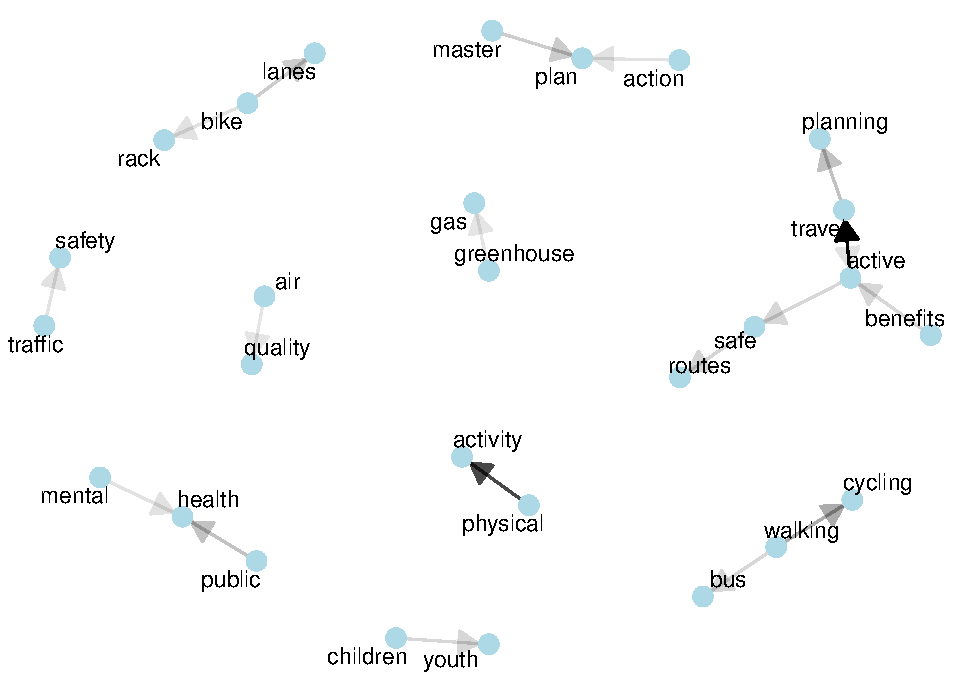
\includegraphics[width=1\linewidth]{AST-Framing-Ontario_files/figure-latex/city-visual-1} 

}

\caption{\label{fig:city-visual}Most common bigrams found in the municipal and regional government documents.}\label{fig:city-visual}
\end{figure}

\begin{figure}

{\centering 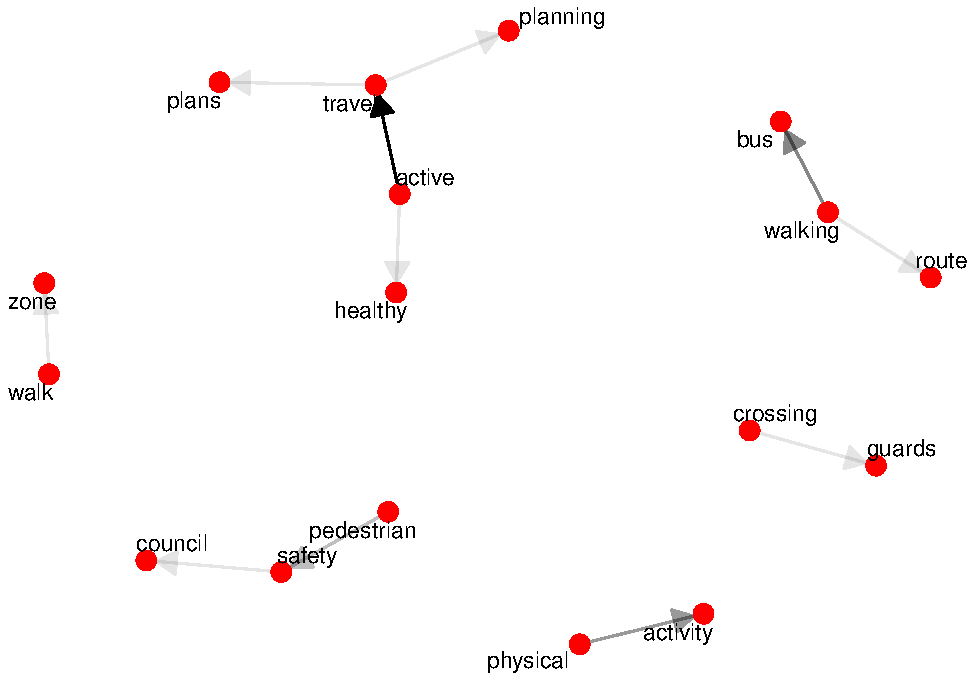
\includegraphics[width=1\linewidth]{AST-Framing-Ontario_files/figure-latex/consortia-visual-1} 

}

\caption{\label{fig:consortia-visual}Most common bigrams found in the transportation consortia documents.}\label{fig:consortia-visual}
\end{figure}

\begin{figure}

{\centering 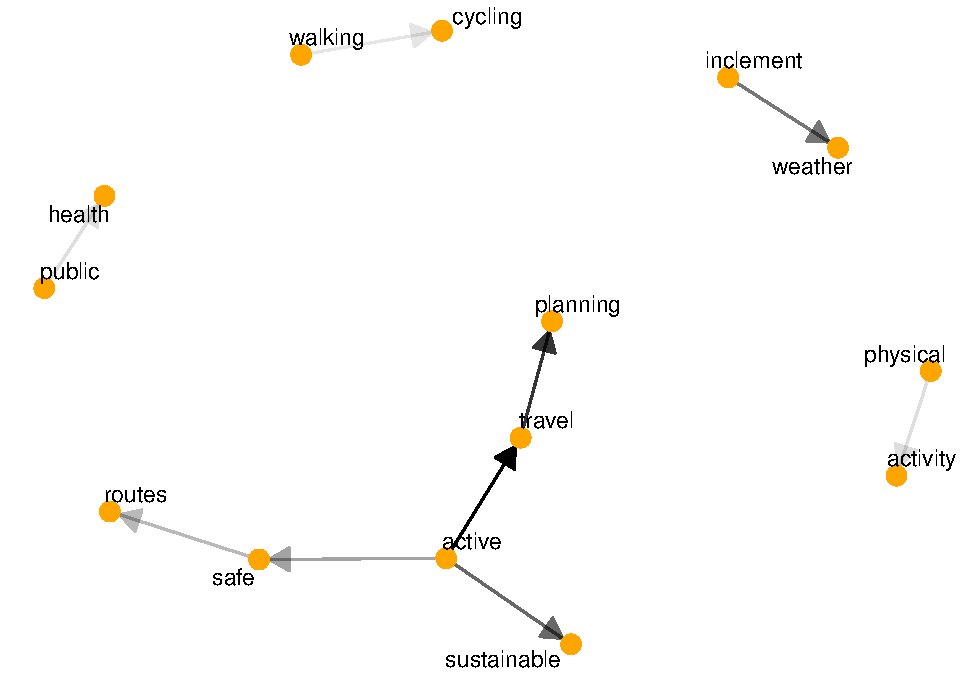
\includegraphics[width=1\linewidth]{AST-Framing-Ontario_files/figure-latex/school-visual-1} 

}

\caption{\label{fig:school-visual}Most common bigrams found in the school board documents.}\label{fig:school-visual}
\end{figure}

\begin{figure}

{\centering 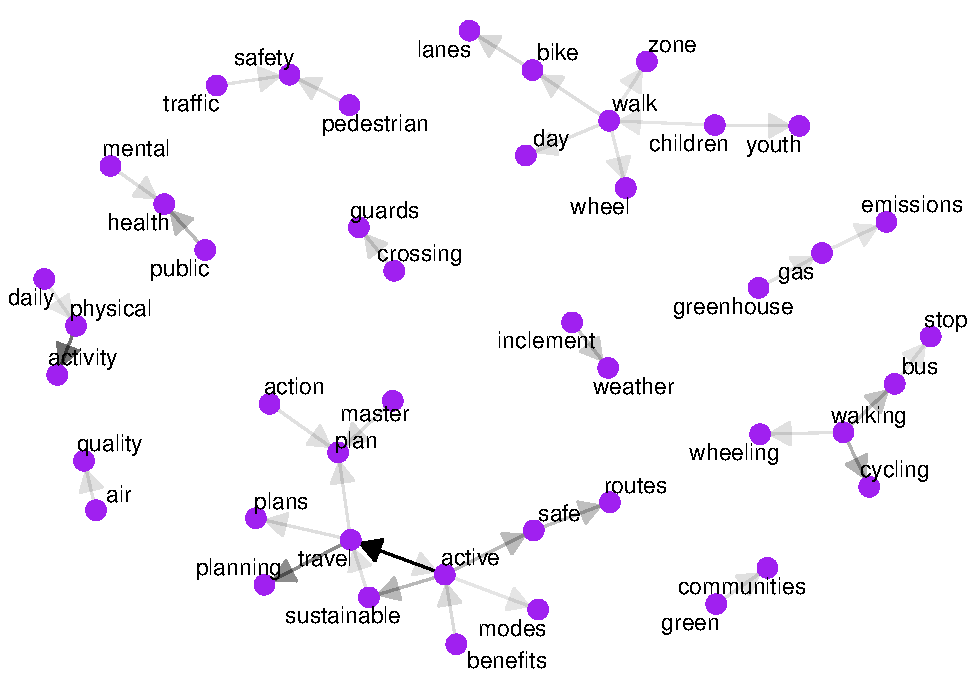
\includegraphics[width=1\linewidth]{AST-Framing-Ontario_files/figure-latex/policy-visual-1} 

}

\caption{\label{fig:policy-visual}Most common bigrams found across all policy documents (i.e., school board, municipality, and transportation consortia combined).}\label{fig:policy-visual}
\end{figure}

We then combined all municipality, school board, and transportation
consortia documents into one ``policy+practice'' corpus. This enabled us
to examine and visualize the most common bigrams found across all of the
material in Ontario that was collected for this study. Figure
\ref{fig:policy-visual} shows all of the bigrams that occur more than 10
times in the policy+practice corpus. In addition to the bigrams already
identified above, we also found \emph{mental health}, \emph{walk day},
and \emph{green communities} as common pairs of consecutive words.
\emph{Green Communities Canada} is a non-profit organization that has
significantly supported AST initiatives through the Ontario Active
School Travel program so the high frequency of this term in the
policy+practice corpus is not surprising. Overall, the policy documents
from STP stakeholder groups seem to focus on four key areas: i) benefits
or impacts of AST; ii) mechanisms of intervention; iii) concerns or
barriers; and iv) supports for AST. This interpretation indicates that
the general public accessing information about AST in Ontario is
informed about a wide range of content related to this issue.

Next, we analyzed bigrams in the academic corpus separately to make
comparisons with the policy+practice corpus. Figure
\ref{fig:academic-visual} indicates that academic papers include several
common bigrams that were also found in the policy documents including
\emph{physical activity} (n = 1566), which is the top bigram,
\emph{traffic safety} (n = 308), and \emph{safe routes} (n = 268).
However, many other factors are identified in the research literature
that are not presented to the general public through policy documents.
After \emph{physical activity}, \emph{built environment} (n = 1175),
\emph{independent mobility} (n = 774), and \emph{urban form} (n = 352)
are the most frequent pairs of consecutive words. Academic papers also
often discuss \emph{distance home} (n = 258), \emph{car ownership} (n =
254), \emph{household income} (n = 254), and \emph{population density}
(n = 205), which are factors that have been found to influence AST. Many
papers also investigate gender differences in AST given that \emph{boys
girls} (n = 211) is another common bigram. Finally, the presence of
\emph{statistically significant} among the top bigrams indicates that
researchers often aim to identify associations using statistical
measures. We found that the academic corpus focuses on a greater range
of topics than found in the policy+practice documents.

\begin{figure}

{\centering 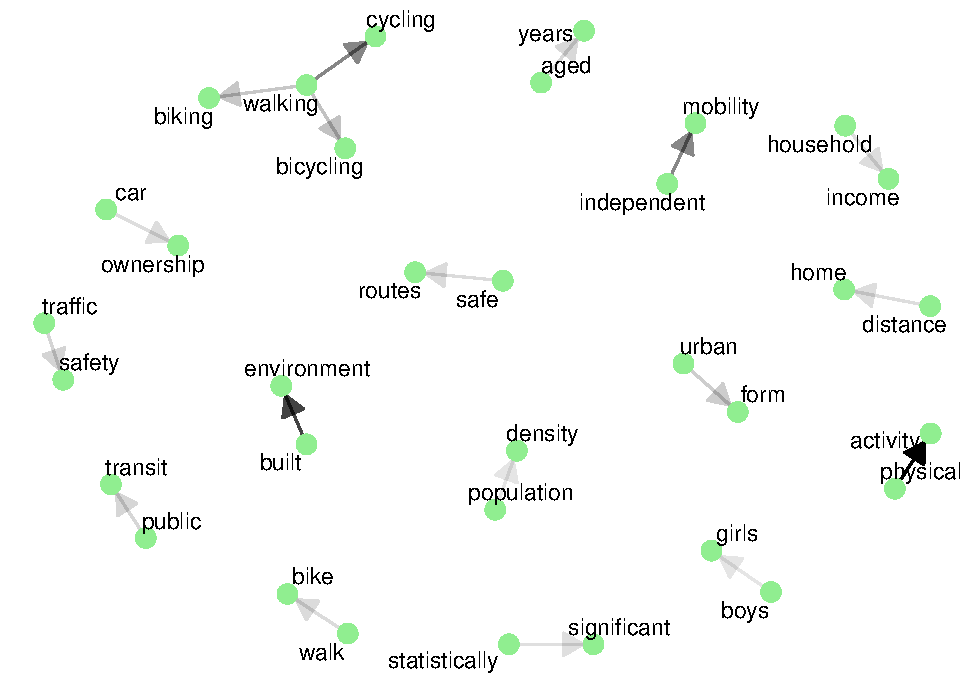
\includegraphics[width=1\linewidth]{AST-Framing-Ontario_files/figure-latex/academic-visual-1} 

}

\caption{\label{fig:academic-visual}Most common bigrams found in the academic papers.}\label{fig:academic-visual}
\end{figure}

We interpreted the most common bigrams from the policy+practice corpus
(see Figure \ref{fig:policy-visual}), which includes all documents from
municipalities, transportation consortia, and school boards, as the main
ideas that STP stakeholder groups focus on and communicate to the public
about AST. We then examined the context of these key ideas by extracting
words-in-context from the corpora. Table \ref{tab:policy-concordance}
presents some examples from select policy documents that illustrate how
the most common bigrams are communicated to the public.

\begin{table}

\caption{\label{tab:content-table}\label{tab:policy-concordance}The context of key terms that were identified as common bigrams.}
\centering
\begin{tabular}[t]{>{}ll>{\raggedright\arraybackslash}p{20em}}
\toprule
Terms & Stakeholder & Context\\
\midrule
\textbf{\cellcolor{gray!6}{Air Quality}} & \cellcolor{gray!6}{School Board} & \cellcolor{gray!6}{Active transportation [...] improves air quality.}\\
\textbf{Benefit} & Municipality & Stronger bones and muscles, improved self-esteem and sense of well-being while reducing stress and risk of chronic disease all benefit those who use active transportation.\\
\textbf{\cellcolor{gray!6}{Walking School Bus}} & \cellcolor{gray!6}{School Board} & \cellcolor{gray!6}{While taking part in a walking school bus, your child will enjoy seeing friends on the way to school. They will be active more often. This is also a great opportunity for your child to socialize with school friends in a monitored and safe way where they can practice social distancing, modelled by a leader.}\\
\textbf{Community} & School Board & Help your students get started on the right foot - encourage them to walk or bike to school when possible. Even leaving the car a block or two and walking the rest of the way helps. It’s good for the environment and your health, and teaches your child independence and community awareness.\\
\textbf{\cellcolor{gray!6}{Emissions}} & \cellcolor{gray!6}{Consortia} & \cellcolor{gray!6}{An active school commute also reduces congestion in school zones and contributes to reducing greenhouse gas emissions – it’s a win-win for everyone!}\\
\addlinespace
\textbf{Health} & Municipality & Active School Travel allows school-aged children the chance to participate in moderate to intense physical activity. This is linked with lower body mass index and improved cardiovascular health.\\
\textbf{\cellcolor{gray!6}{Lanes}} & \cellcolor{gray!6}{Municipality} & \cellcolor{gray!6}{We are continuing to build on the cycling and pedestrian network by adding more bike lanes, building multi-use paths and encouraging developments to provide better pedestrian/cycling environments.}\\
\textbf{Mental Health} & Municipality & Active and Sustainable School Travel (ASST) not only improves physical and mental health but contributes to a healthier environment and safer streets.\\
\textbf{\cellcolor{gray!6}{Physical Health}} & \cellcolor{gray!6}{Municipality} & \cellcolor{gray!6}{Encouraging Active Transportation promotes physical health and recreation, helps manage congestion, reduces emissions and supports municipal objectives for efficient land use.}\\
\bottomrule
\end{tabular}
\end{table}

\hypertarget{topic-modelling}{%
\subsection{5.3. Topic modelling}\label{topic-modelling}}

\begin{figure}
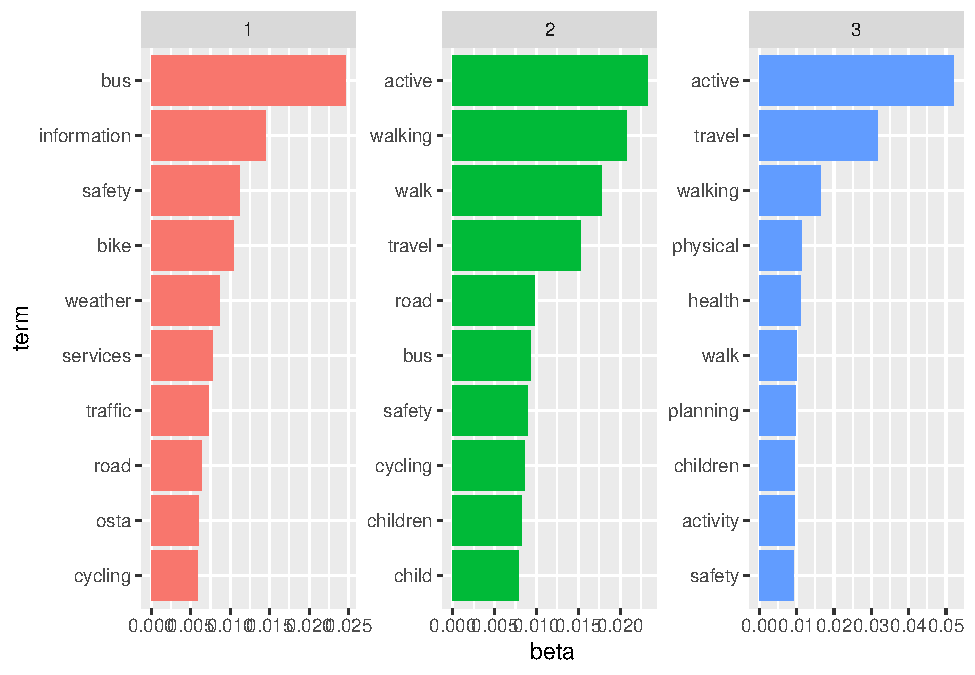
\includegraphics[width=1\linewidth]{AST-Framing-Ontario_files/figure-latex/policy-terms-1} \caption{\label{fig:policy-terms}Topics identified in the policy+practice corpus according to clusters of words. The per-word-per-topic probabilities are shown by beta.}\label{fig:policy-terms}
\end{figure}

\begin{figure}
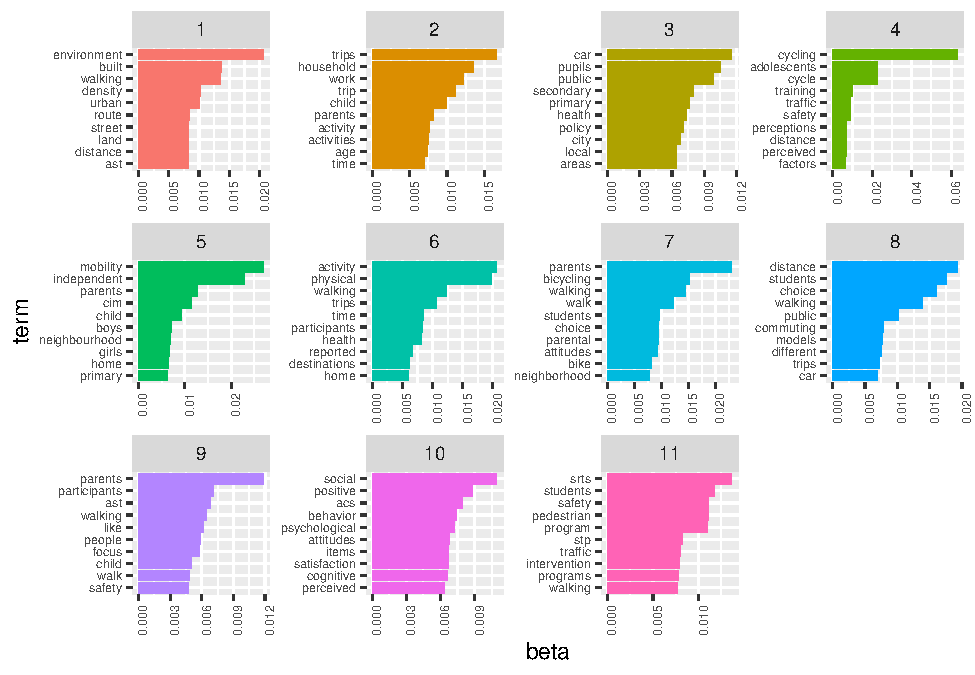
\includegraphics[width=1\linewidth]{AST-Framing-Ontario_files/figure-latex/academic-terms-1} \caption{\label{fig:academic-terms}Topics identified in the academic corpus according to clusters of words. The per-word-per-topic probabilities are shown by beta.}\label{fig:academic-terms}
\end{figure}

For the final part of our analysis, we conducted topic modelling to
examine the different topics found in the policy and academic corpora.
We focused on the policy/practice corpus, instead of assessing the
municipal, school, and consortia documents separately, so that we could
report on the various frames used across all documents put out by STP
stakeholder groups in Ontario. We then estimated Latent Dirichlet
Allocation (LDA) models for each corpus. Parameter tuning suggests that
the policy+practice corpus has between 9 and 13 topics and the academic
corpus has between 17 and 25 topics. After running the LDA model for the
academic corpus, we realized the difficulty of interpreting a minimum of
17 topics based on the clusters of words that were identified. We
experimented with the model by adjusting the number of topics and
evaluating the output of terms in each topic. We found that there were 9
distinct topics that could be interpreted in the policy corpus and 11
topics in the academic corpus, after which there was too much overlap
for the clusters to be meaningfully interpreted. Figures
\ref{fig:policy-terms} and \ref{fig:academic-terms} present the main
terms that are associated with the topics found in each corpus.

In the policy+practice corpus, we identified the following topics based
on the cluster of words: (1) safety; (2) weather and busing; (3) active
travel planning; (4) walking; (5) resources for walking; (6) bicycling;
(7) active travel concerns; (8) benefits of active travel; and (9)
busing logistics. These topics indicate that STP stakeholder groups are
sending the message that walking and bicycling to school are healthy
travel modes for students, particularly in terms of physical activity.
We also found that information is shared to support parents and students
in using active modes to school, for example regarding the availability
of bicycling lanes and tips for route choice for walking.

The academic corpus has a higher number of topics likely due to the
volume of papers included. The following topics were identified based on
the clusters of words: (1) physical activity; (2) safe routes to school
for active travel; (3) behaviours and attitudes; (4) bicycling; (5)
walking; (6) built environment; (7) trip choice; (8) active school
travel interventions; (9) parents; (10) children's independent mobility;
and (11) public health and policies. This corpus reflects a broader
range of topics than the policy/practice corpus.

\hypertarget{frames}{%
\subsection{5.4. Frames}\label{frames}}

Based on the identified bigrams and topics, we determined that the
policy+practice corpus primarily frames AST as a health and
environmental issue. STP stakeholder groups appear to position walking,
bicycling, or rolling to school as beneficial to individual health, via
physical activity and improved mental health, and to the broader
community through a reduction in traffic and vehicle emissions. Here, we
present some examples from the policy documents that illustrate how the
health and environmental frame is communicated:

\begin{quote}
\emph{If you live in a walk zone, the best way to get to school is by
walking or biking. This promotes physical activity, helps the
environment and minimizes traffic around schools during busy times.}
(City of Barrie)
\end{quote}

\begin{quote}
\emph{Active school travel is a great way for children to be physically
active, which is associated with improved physical and mental health,
while making school zones safer, by reducing traffic volumes at and
around schools.}(Region of Leeds, Grenville and Lanark)
\end{quote}

\begin{quote}
\emph{The WCDSB supports active transportation as the preferred method
of transportation to school because it is a healthy choice that has
proven links to greater student achievement.} (Waterloo Catholic
District School Board)
\end{quote}

Furthermore, we found that policy documents make claims about the
benefits of AST that are consistent with the findings of academic
research and evaluation.

\begin{quote}
\emph{For their health, safety, environment and community: Kids learn
healthy habits and concentrate better in class; One less car (yours)
reduces traffic and parking problems in school zones; Teach your kids
about traffic safety; Start a walking school bus; your kids make friends
in every grade, and that can prevent bullying.} (City of Guelph)
\end{quote}

\begin{quote}
\emph{There are lots of benefits in the classroom for children that walk
or cycle to school on a regular basis. Some of these benefits include
improved concentration and better coping with stress. Being outside
helps to prevent feelings of isolation and increases their social
interactions. Walking and biking to school can also save you money and
lead to fewer cars on the road.} (City of Ottawa)
\end{quote}

The secondary frame in policy documents is that AST is accessible and
feasible for children and parents. Despite the emphasis on the logistics
of busing in the topic modelling, the documents indicate that there is
an opportunity for or prospect of behaviour change. Some cities and
schools explain how children and parents can leave the car at home and
make the journey to school on foot or by bike. This frame encourages the
public to evaluate their own travel decisions and to access resources
(e.g., walking skills checklist) that will help them make AST a first
choice. Examples of this secondary frame include:

\begin{quote}
\emph{A way to make sure your child is safe while walking to school is
with a `walking school bus.' Here are some tips for a walking school
bus: Invite families who live nearby to walk; Pick a route and take a
test walk; Take side streets and paths that are less busy with traffic;
Decide how often the group will walk together; Talk with your boss to
adjust your day; Have fun!} (City of Ottawa)
\end{quote}

\begin{quote}
\emph{Help your students get started on the right foot - encourage them
to walk or bike to school when possible. Even leaving the car a block or
two and walking the rest of the way helps. It's good for the environment
and your health, and teaches your child independence and community
awareness.} (Halton District School Board)
\end{quote}

\begin{quote}
\emph{Want to boost your child's mental and physical health? Ottawa
Public Health, City of Ottawa, and OSTA have produced a tipsheet for
parents about ``active transportation'' to school -- fitting walking and
wheeling into your daily routine.} (Ottawa-Carleton District School
Board)
\end{quote}

Finally, both AST frames present solutions to encourage AST. STP
stakeholder groups seem to be communicating that AST is a healthy and
easy option as a result of policy changes (e.g., available resources for
parents and children) and improvements to the built environment. This
could include examples of various efforts that are underway to support
AST including route planning.

\begin{quote}
\emph{School Travel Planning is a community-based approach that aims to
increase the number of students and adults choosing active and
sustainable travel to get to and from school. This approach addresses
concerns about safety, physical activity, and the environment.} (City of
Hamilton)
\end{quote}

\begin{quote}
\emph{Today, as more and more of our neighbourhoods are being
retrofitted with new sidewalks and bike lanes, pedestrian crossovers,
street lights, reduced speed limits and/or crossing guards, the walk or
bike ride to and from school has never been easier, safer or healthier.}
(Hamilton-Wentworth District Catholic School Board)
\end{quote}

\hypertarget{discussion}{%
\section{6. Discussion}\label{discussion}}

\hypertarget{current-ast-frames-in-ontario}{%
\subsection{6.1. Current AST frames in
Ontario}\label{current-ast-frames-in-ontario}}

Using natural language processing techniques, we analyzed how AST is
framed in 69 documents available to the public on the websites of STP
stakeholder groups in Ontario. Two main frames in the policy+practice
corpus were identified based on the most common bigrams and topics from
the LDA model.

We found that AST is primarily framed to parents as beneficial to the
health and wellbeing of children and to environmental sustainability.
The policy documents reflect the evidence that AST contributes
positively to children's physical health (see Faulkner et al., 2009;
Schoeppe et al., 2015), although the statements regarding the benefits
of AST to children's school performance are less well-supported in the
extant literature (Westman et al., 2020). STP stakeholder groups also
communicate that increasing AST may reduce traffic near and around
schools. This is conveyed presumably to alleviate parental concerns
about traffic and safety (Evers et al., 2014; Mammen et al., 2012;
Rothman et al., 2015; Wilson et al., 2018) or to reduce the frequency of
risky behaviours from drivers around schools (Rothman et al., 2017).

In the secondary frame, AST is presented as an accessible and feasible
way for children to travel to and from school. Children and parents are
encouraged to adopt new travel behaviours. STP stakeholder groups
identified different ways that parents could encourage or support their
children to commute to school by using active modes. Some school boards
and municipalities also shared resources such as walking tip sheets and
guidance for starting a walking school bus. Other advice included
dropping children off one or two blocks away from school so that they
could walk or bike part of the trip. The general emphasis of this frame
is communicating information that could change parental perceptions
about the ease of their children using active modes to school, which may
be seen by STP stakeholder groups as a ``modifiable'' factor (see Riazi
et al., 2019). In turn, this could encourage parents to modify their
routines and incorporate opportunities for their children to use active
modes to school.

Both frames present the AST issue in a positive light. Neither frame
appears to explain why declining rates of AST are a problem or convey
any urgency to this issue so that it attracts the attention of parents,
the general public, or policy makers. Communicating the potential
outcomes of increased AST may be persuasive arguments to motivate
behaviour change, but these frames do not seem to encourage parents or
the general public to view their current behaviour as problematic or
unhealthy for their children's development and their community. Thus,
behaviour change is presented as an option for some but not an
imperative for all. For example, parents who drive their children to
school have reported concerns about traffic volume around schools
(Mammen et al., 2012), but may not recognize that their own behaviour
contributes to the problem that is perceived to prevent their child from
safely walking or bicycling to school (Collins and Kearns, 2001).
Reynard et al. (2021) similarly found in their analysis of Canadian
municipal documents that one of the dominant frames presented the
adoption of behaviours to help mitigate the climate crisis as a choice
but not ``the expected norm.''

We found that the proposed solutions in the secondary frame to increase
AST align with different levels of the socioecological model: 1)
behaviour change from individuals or households making different travel
decisions; 2) policies like STP that create resources for AST; and 3)
engineering solutions like bicycle lanes. This reflects findings from
the AST literature that a range of solutions are needed to address
different factors that influence AST (\emph{inter alia, see} Mitra,
2013; Panter et al., 2010). The recognition of engineering changes may
reflect the strong engagement of the ``policy stream'' (Kingdon, 1984)
since engineering staff and municipal representatives are common STP
stakeholders in Canada (Buttazzoni et al., 2018; Mammen et al., 2015),
as well as the evidence that the built environment influences mode
choice to school. However, it is beyond the scope of this paper to
assess whether the proposed solutions are perceived to be sufficient by
parents for increasing AST.

\hypertarget{implications-for-school-travel-planning}{%
\subsection{6.2. Implications for school travel
planning}\label{implications-for-school-travel-planning}}

STP stakeholders should problematize the significant decline in AST that
has occurred over recent decades in Canada and emphasize that this issue
merits urgent behaviour change. A study investigating the influence of
different valence framings of CO2 emissions on transport mode shift
found that positive framing can be less effective than negative framing
(Waygood and Avineri, 2018). A negative framing that challenges the
social norm of driving could be more motivational to shift modes, which
would be consistent with other findings (see Waygood and Avineri, 2018).
Policy documents should make it clear that continued use of nonactive
modes to school can deprive children of opportunities to increase
physical activity and to gain health and social benefits.

There is a noticeable lack of focus on certain household determinants of
AST in the two frames that needs to be addressed. For example, the role
of convenience and inclement weather in shaping household travel
decisions (Buliung et al., 2011) and the complexity of travel
arrangements that must be coordinated by households (see Buliung et al.,
2021) were not found to be discussed. The desire to escort children to
school, which has been noted by parents as a reason to continue driving
(Westman et al., 2017a), is also not adequately addressed by STP
stakeholders. Parental assessment of a child's ability to undertake the
journey to school was likewise overlooked despite its role in decision
making for mode choice to school (Faulkner et al., 2010). Framing AST as
a developmental opportunity or a rite of passage that children have been
denied could challenge the prevailing culture of risk avoidance which
discourages parents from letting their children use active modes to
school.

Future research and evaluation by STP stakeholders should investigate
how parents or the general public respond to messages or information
that encourages the adoption of AST and evaluate which are most
effective. It would be helpful to understand which frames would most
encourage behaviour change or increase political support for
interventions that address barriers to AST. This type of information
could ensure that educational strategies and promotional materials
increase buy-in for their target audience. If Canadian STP stakeholders
wish to involve more local residents in their efforts (Buttazzoni et
al., 2018), it would also be worthwhile for them to produce different
materials that communicate why this issue is important to the general
public, regardless of whether they currently have children commuting
to/from school.

\hypertarget{limitations}{%
\subsection{6.3. Limitations}\label{limitations}}

A limitation of this study is that we only analyzed English-language
texts that were easily accessible to the general public on the websites
of STP stakeholders in Ontario. We did not include French-language
materials from Ontario's 12 French school boards (a mixture of public
and Catholic schools). Parents likely receive information about AST
directly from schools, which may contain more content that reflects the
local barriers to AST, but these materials were not used in our
analysis.

\hypertarget{conclusion}{%
\section{7. Conclusion}\label{conclusion}}

We used natural language processing techniques to examine how different
school travel planning (STP) stakeholders in Ontario frame the issue of
AST. STP stakeholders frame AST as an accessible and feasible way to
travel to school that is valuable to children's health and to the
environment. STP stakeholders are communicating that this issue can be
addressed through household behaviour change and policy solutions.
Policy documents reveal that STP stakeholders are focusing on
``modifiable factors'' such as parental perceptions or micro-scale
elements in the built environment to increase rates of AST. However, AST
may not be framed sufficiently as a ``problem'' that requires urgent
intervention, which may impact how parents respond to behaviour change
initiatives and limit awareness in the general public. In their public
materials about AST, STP stakeholders should emphasize why AST rates
should increase in local communities and how the negative effects of
nonactive modes to school may impact children's health and wellbeing.

\hypertarget{acknowledgments}{%
\section{Acknowledgments}\label{acknowledgments}}

This research was completed using open software, and the authors wish to
acknowledge the developers of the following \texttt{R} packages:
\texttt{dplyr} (Wickham et al., 2021b), \texttt{ggraph} (Pedersen,
2021), \texttt{ggplot2} (Wickham et al., 2021a), \texttt{igraph} (file.,
2022), \texttt{pdftools} (Ooms, 2021), \texttt{readr} (Wickham et al.,
2021c), \texttt{reshape2} (Wickham, 2020), \texttt{stringr} (Wickham,
2019), \texttt{text2vec} (Selivanov et al., 2020), \texttt{textdata}
(Hvitfeldt, 2020), \texttt{tidyr} (Wickham, 2021), \texttt{tidytext}
(Robinson and Silge, 2021), \texttt{tm} (Feinerer and Hornik, 2020),
\texttt{tools} (\textbf{R-tools?}), \texttt{topicmodels} (Grün and
Hornik, 2021), \texttt{widyr} (Robinson, 2021), \texttt{word2vec}
(Wijffels, 2021), \texttt{wordcloud} (Fellows, 2018),
\texttt{DiagrammeR} (\textbf{R-diagrammeR?}), and \texttt{kableextra}
(\textbf{R-kableextra?}).

\hypertarget{references}{%
\section*{References}\label{references}}
\addcontentsline{toc}{section}{References}

\hypertarget{refs}{}
\begin{CSLReferences}{1}{0}
\leavevmode\vadjust pre{\hypertarget{ref-albalawiUsingTopicModeling2020}{}}%
Albalawi, R., Yeap, T.H., Benyoucef, M., 2020. Using topic modeling
methods for short-text data: A comparative analysis. Frontiers in
Artificial Intelligence 3, 42.
doi:\href{https://doi.org/10.3389/frai.2020.00042}{10.3389/frai.2020.00042}

\leavevmode\vadjust pre{\hypertarget{ref-badlandDevelopmentSystemsModel2016}{}}%
Badland, H., Kearns, R., Carroll, P., Oliver, M., Mavoa, S., Donovan,
P., Parker, K., Chaudhury, M., Lin, E.-Y., Witten, K., 2016. Development
of a systems model to visualise the complexity of children's independent
mobility. Children's Geographies 14, 91--100.
doi:\href{https://doi.org/10.1080/14733285.2015.1021240}{10.1080/14733285.2015.1021240}

\leavevmode\vadjust pre{\hypertarget{ref-borrestadExperiencesRandomisedControlled2012}{}}%
Børrestad, L.A.B., Østergaard, L., Andersen, L.B., Bere, E., 2012.
Experiences from a randomised, controlled trial on cycling to school:
Does cycling increase cardiorespiratory fitness? Scandinavian Journal of
Public Health 40, 245--252.
doi:\href{https://doi.org/10.1177/1403494812443606}{10.1177/1403494812443606}

\leavevmode\vadjust pre{\hypertarget{ref-brunsdon2020opening}{}}%
Brunsdon, C., Comber, A., 2020. Opening practice: Supporting
reproducibility and critical spatial data science. Journal of
Geographical Systems.
doi:\href{https://doi.org/10.1007/s10109-020-00334-2}{10.1007/s10109-020-00334-2}

\leavevmode\vadjust pre{\hypertarget{ref-buliungSchoolTravelPlanning2011}{}}%
Buliung, R., Faulkner, G., Beesley, T., Kennedy, J., 2011. School travel
planning: Mobilizing school and community resources to encourage active
school transportation. Journal of School Health 81, 704--712.
doi:\href{https://doi.org/10.1111/j.1746-1561.2011.00647.x}{10.1111/j.1746-1561.2011.00647.x}

\leavevmode\vadjust pre{\hypertarget{ref-buliungLivingJourneySchool2021}{}}%
Buliung, R., Hess, P., Flowers, L., Moola, F.J., Faulkner, G., 2021.
Living the journey to school: Conceptual asymmetry between parents and
planners on the journey to school. Social Science \& Medicine 284,
114237.
doi:\href{https://doi.org/10.1016/j.socscimed.2021.114237}{10.1016/j.socscimed.2021.114237}

\leavevmode\vadjust pre{\hypertarget{ref-buttazzoniPromotingActiveSchool2019}{}}%
Buttazzoni, A.N., Clark, A.F., Seabrook, J.A., Gilliland, J.A., 2019.
Promoting active school travel in elementary schools: A regional case
study of the school travel planning intervention. Journal of Transport
\& Health 12, 206--219.
doi:\href{https://doi.org/10.1016/j.jth.2019.01.007}{10.1016/j.jth.2019.01.007}

\leavevmode\vadjust pre{\hypertarget{ref-buttazzoniSupportingActiveSchool2018}{}}%
Buttazzoni, A.N., Coen, S.E., Gilliland, J.A., 2018. Supporting active
school travel: A qualitative analysis of implementing a regional safe
routes to school program. Social Science \& Medicine 212, 181--190.
doi:\href{https://doi.org/10.1016/j.socscimed.2018.07.032}{10.1016/j.socscimed.2018.07.032}

\leavevmode\vadjust pre{\hypertarget{ref-GreenCommunities2016}{}}%
Canada, G.C., 2020. Ontario active school travel {[}WWW Document{]}. URL
\url{https://ontarioactiveschooltravel.ca/about-ontario-active-school-travel/}

\leavevmode\vadjust pre{\hypertarget{ref-GreenCommunitiesProjects}{}}%
Canada, G.C., 2021. Ontario active school travel fund {[}WWW
Document{]}. URL
\url{https://ontarioactiveschooltravel.ca/ontario-active-school-travel-fund/}

\leavevmode\vadjust pre{\hypertarget{ref-TACbikeinfra2020}{}}%
Canada, T.A. of, 2020. Safety performance of bicycle infrastructure in
canada {[}WWW Document{]}. URL
\url{https://www.tac-atc.ca/en/publications/ptm-spbi-e}

\leavevmode\vadjust pre{\hypertarget{ref-chenPromotingActiveStudent2018}{}}%
Chen, P., Jiao, J., Xu, M., Gao, X., Bischak, C., 2018. Promoting active
student travel: A longitudinal study. Journal of Transport Geography 70,
265--274.
doi:\href{https://doi.org/10.1016/j.jtrangeo.2018.06.015}{10.1016/j.jtrangeo.2018.06.015}

\leavevmode\vadjust pre{\hypertarget{ref-collinsSafeJourneysEnterprising2001}{}}%
Collins, D.C.A., Kearns, R.A., 2001. The safe journeys of an
enterprising school: Negotiating landscapes of opportunity and risk.
Health \& Place 7, 293--306.
doi:\href{https://doi.org/10.1016/S1353-8292(01)00021-1}{10.1016/S1353-8292(01)00021-1}

\leavevmode\vadjust pre{\hypertarget{ref-demeesterParentalPerceivedNeighborhood2014}{}}%
De Meester, F., Van Dyck, D., De Bourdeaudhuij, I., Cardon, G., 2014.
Parental perceived neighborhood attributes: Associations with active
transport and physical activity among 10-12 year old children and the
mediating role of independent mobility. BMC public health 14, 631.
doi:\href{https://doi.org/10.1186/1471-2458-14-631}{10.1186/1471-2458-14-631}

\leavevmode\vadjust pre{\hypertarget{ref-depouxCommunicatingClimateChange2017}{}}%
Depoux, A., Hémono, M., Puig-Malet, S., Pédron, R., Flahault, A., 2017.
Communicating climate change and health in the media. Public Health
Reviews 38, 7.
doi:\href{https://doi.org/10.1186/s40985-016-0044-1}{10.1186/s40985-016-0044-1}

\leavevmode\vadjust pre{\hypertarget{ref-eversParentSafetyPerceptions2014}{}}%
Evers, C., Boles, S., Johnson-Shelton, D., Schlossberg, M., Richey, D.,
2014. Parent safety perceptions of child walking routes. Journal of
Transport \& Health 1, 108--115.
doi:\href{https://doi.org/10.1016/j.jth.2014.03.003}{10.1016/j.jth.2014.03.003}

\leavevmode\vadjust pre{\hypertarget{ref-farberRunning2011}{}}%
Farber, S., Páez, A., 2011. Running to stay in place: The time-use
implications of automobile oriented land-use and travel. Journal of
Transport Geography 19, 782--793.
doi:\href{https://doi.org/10.1016/j.jtrangeo.2010.09.008}{10.1016/j.jtrangeo.2010.09.008}

\leavevmode\vadjust pre{\hypertarget{ref-faulknerActiveSchoolTransport2009}{}}%
Faulkner, G.E.J., Buliung, R.N., Flora, P.K., Fusco, C., 2009. Active
school transport, physical activity levels and body weight of children
and youth: A systematic review. Preventive Medicine 48, 3--8.
doi:\href{https://doi.org/10.1016/j.ypmed.2008.10.017}{10.1016/j.ypmed.2008.10.017}

\leavevmode\vadjust pre{\hypertarget{ref-faulknerWhatQuickestEasiest2010}{}}%
Faulkner, G.E., Richichi, V., Buliung, R.N., Fusco, C., Moola, F., 2010.
What's "quickest and easiest?": Parental decision making about school
trip mode. International Journal of Behavioral Nutrition and Physical
Activity 7, 1--11.
doi:\href{https://doi.org/10.1186/1479-5868-7-62}{10.1186/1479-5868-7-62}

\leavevmode\vadjust pre{\hypertarget{ref-faulknerSchoolTravelChildren2013}{}}%
Faulkner, G., Stone, M., Buliung, R., Wong, B., Mitra, R., 2013. School
travel and children's physical activity: A cross-sectional study
examining the influence of distance. BMC public health 13, 1166.
doi:\href{https://doi.org/10.1186/1471-2458-13-1166}{10.1186/1471-2458-13-1166}

\leavevmode\vadjust pre{\hypertarget{ref-R-tm}{}}%
Feinerer, I., Hornik, K., 2020. Tm: Text mining package.

\leavevmode\vadjust pre{\hypertarget{ref-R-wordcloud}{}}%
Fellows, I., 2018. Wordcloud: Word clouds.

\leavevmode\vadjust pre{\hypertarget{ref-R-igraph}{}}%
file., S.A., 2022. Igraph: Network analysis and visualization.

\leavevmode\vadjust pre{\hypertarget{ref-fuscoUnderstandingChildrenPerceptions2012}{}}%
Fusco, C., Moola, F., Faulkner, G., Buliung, R., Richichi, V., 2012.
Toward an understanding of children's perceptions of their transport
geographies: (Non)active school travel and visual representations of the
built environment. Journal of Transport Geography, Special {section On
Child} \& {Youth Mobility} 20, 62--70.
doi:\href{https://doi.org/10.1016/j.jtrangeo.2011.07.001}{10.1016/j.jtrangeo.2011.07.001}

\leavevmode\vadjust pre{\hypertarget{ref-gamsonChangingCulture1987}{}}%
Gamson, W.A., Modigliani, A., 1987. The changing culture of affirmative
action, in: Waygood, E.O.D., Friman, M., Olsson, L.E., Mitra, R. (Eds.),
Research in Political Sociology. {JAI Press}, pp. 137--177.

\leavevmode\vadjust pre{\hypertarget{ref-goffmanFrameAnalysisEssay1974}{}}%
Goffman, E., 1974. Frame analysis: An essay on the organization of
experience, Frame analysis: {An} essay on the organization of
experience. {Harvard University Press}, {Cambridge, MA, US}.

\leavevmode\vadjust pre{\hypertarget{ref-R-topicmodels}{}}%
Grün, B., Hornik, K., 2021. Topicmodels: Topic models.

\leavevmode\vadjust pre{\hypertarget{ref-R-textdata}{}}%
Hvitfeldt, E., 2020. Textdata: Download and load various text datasets.

\leavevmode\vadjust pre{\hypertarget{ref-ikedaAssociationsChildrenActive2018}{}}%
Ikeda, E., Hinckson, E., Witten, K., Smith, M., 2018. Associations of
children's active school travel with perceptions of the physical
environment and characteristics of the social environment: A systematic
review. Health \& Place 54, 118--131.
doi:\href{https://doi.org/10.1016/j.healthplace.2018.09.009}{10.1016/j.healthplace.2018.09.009}

\leavevmode\vadjust pre{\hypertarget{ref-jacobiQuantitativeAnalysisLarge2016}{}}%
Jacobi, C., van Atteveldt, W., Welbers, K., 2016. Quantitative analysis
of large amounts of journalistic texts using topic modelling. Digital
Journalism 4, 89--106.
doi:\href{https://doi.org/10.1080/21670811.2015.1093271}{10.1080/21670811.2015.1093271}

\leavevmode\vadjust pre{\hypertarget{ref-kingdonAgendasAlternativesPublic1984}{}}%
Kingdon, J.W., 1984. Agendas, alternatives, and public policies. {Harper
Collins}.

\leavevmode\vadjust pre{\hypertarget{ref-langUnderstandingModalChoice2011}{}}%
Lang, D., Collins, D., Kearns, R., 2011. Understanding modal choice for
the trip to school. Journal of Transport Geography 19, 509--514.
doi:\href{https://doi.org/10.1016/j.jtrangeo.2010.05.005}{10.1016/j.jtrangeo.2010.05.005}

\leavevmode\vadjust pre{\hypertarget{ref-laroucheRatherBikeSchool2016}{}}%
Larouche, R., Stone, M., Buliung, R.N., Faulkner, G., 2016. ''I'd rather
bike to school!'': Profiling children who would prefer to cycle to
school. Journal of Transport \& Health 3, 377--385.
doi:\href{https://doi.org/10.1016/j.jth.2016.06.010}{10.1016/j.jth.2016.06.010}

\leavevmode\vadjust pre{\hypertarget{ref-larsenRouteBasedAnalysisCapture2012}{}}%
Larsen, K., Gilliland, J., Hess, P.M., 2012. Route-based analysis to
capture the environmental influences on a child's mode of travel between
home and school. Annals of the Association of American Geographers 102,
1348--1365.

\leavevmode\vadjust pre{\hypertarget{ref-mahFramecriticalPolicyAnalysis2014}{}}%
Mah, C.L., Hamill, C., Rondeau, K., McIntyre, L., 2014. A frame-critical
policy analysis of canada's response to the world food summit
1998\textendash 2008. Archives of Public Health 72, 41.
doi:\href{https://doi.org/10.1186/2049-3258-72-41}{10.1186/2049-3258-72-41}

\leavevmode\vadjust pre{\hypertarget{ref-mahDoesParentalSupport2017a}{}}%
Mah, S.K., Nettlefold, L., Macdonald, H.M., Winters, M., Race, D., Voss,
C., McKay, H.A., 2017. Does parental support influence children's active
school travel? Preventive Medicine Reports 6, 346--351.
doi:\href{https://doi.org/10.1016/j.pmedr.2017.04.008}{10.1016/j.pmedr.2017.04.008}

\leavevmode\vadjust pre{\hypertarget{ref-maibachReframingClimateChange2010}{}}%
Maibach, E.W., Nisbet, M., Baldwin, P., Akerlof, K., Diao, G., 2010.
Reframing climate change as a public health issue: An exploratory study
of public reactions. BMC Public Health 10, 1--11.
doi:\href{https://doi.org/10.1186/1471-2458-10-299}{10.1186/1471-2458-10-299}

\leavevmode\vadjust pre{\hypertarget{ref-mammenUnderstandingDriveEscort2012}{}}%
Mammen, G., Faulkner, G., Buliung, R., Lay, J., 2012. Understanding the
drive to escort: A cross-sectional analysis examining parental attitudes
towards children's school travel and independent mobility. BMC public
health 12, 862.
doi:\href{https://doi.org/10.1186/1471-2458-12-862}{10.1186/1471-2458-12-862}

\leavevmode\vadjust pre{\hypertarget{ref-mammenSchoolTravelPlanning2014}{}}%
Mammen, G., Stone, M.R., Buliung, R., Faulkner, G., 2014a. School travel
planning in canada: Identifying child, family, and school-level
characteristics associated with travel mode shift from driving to active
school travel. Journal of Transport \& Health 1, 288--294.
doi:\href{https://doi.org/10.1016/j.jth.2014.09.004}{10.1016/j.jth.2014.09.004}

\leavevmode\vadjust pre{\hypertarget{ref-mammenPuttingSchoolTravel2015}{}}%
Mammen, G., Stone, M.R., Buliung, R., Faulkner, G., 2015. ''Putting
school travel on the map'': Facilitators and barriers to implementing
school travel planning in canada. Journal of Transport \& Health 2,
318--326.
doi:\href{https://doi.org/10.1016/j.jth.2015.05.003}{10.1016/j.jth.2015.05.003}

\leavevmode\vadjust pre{\hypertarget{ref-mammenActiveSchoolTravel2014}{}}%
Mammen, G., Stone, M.R., Faulkner, G., Ramanathan, S., Buliung, R.,
O'Brien, C., Kennedy, J., 2014b. Active school travel: An evaluation of
the canadian school travel planning intervention. Preventive Medicine
60, 55--59.
doi:\href{https://doi.org/10.1016/j.ypmed.2013.12.008}{10.1016/j.ypmed.2013.12.008}

\leavevmode\vadjust pre{\hypertarget{ref-michailChildrenExperiencesTheir2021}{}}%
Michail, N., Ozbil, A., Parnell, R., Wilkie, S., 2021. Children's
experiences of their journey to school: Integrating behaviour change
frameworks to inform the role of the built environment in active school
travel promotion. International Journal of Environmental Research and
Public Health 18, 4992.
doi:\href{https://doi.org/10.3390/ijerph18094992}{10.3390/ijerph18094992}

\leavevmode\vadjust pre{\hypertarget{ref-mitraIndependentMobilityMode2013}{}}%
Mitra, R., 2013. Independent mobility and mode choice for school
transportation: A review and framework for future research. Transport
Reviews 33, 21--43.
doi:\href{https://doi.org/10.1080/01441647.2012.743490}{10.1080/01441647.2012.743490}

\leavevmode\vadjust pre{\hypertarget{ref-R-pdftools}{}}%
Ooms, J., 2021. Pdftools: Text extraction, rendering and converting of
PDF documents.

\leavevmode\vadjust pre{\hypertarget{ref-paezEnjoymentCommuteComparison2010}{}}%
Páez, A., Whalen, K., 2010. Enjoyment of commute: A comparison of
different transportation modes. Transportation Research Part A: Policy
and Practice 44, 537--549.
doi:\href{https://doi.org/10.1016/j.tra.2010.04.003}{10.1016/j.tra.2010.04.003}

\leavevmode\vadjust pre{\hypertarget{ref-panFramingAnalysisApproach1993}{}}%
Pan, Z., Kosicki, G.M., 1993. Framing analysis: An approach to news
discourse. Political Communication 10, 55--75.
doi:\href{https://doi.org/10.1080/10584609.1993.9962963}{10.1080/10584609.1993.9962963}

\leavevmode\vadjust pre{\hypertarget{ref-panterAttitudesSocialSupport2010}{}}%
Panter, J.R., Jones, A.P., Sluijs, E.M.F. van, Griffin, S.J., 2010.
Attitudes, social support and environmental perceptions as predictors of
active commuting behaviour in school children. Journal of Epidemiology
\& Community Health 64, 41--48.
doi:\href{https://doi.org/10.1136/jech.2009.086918}{10.1136/jech.2009.086918}

\leavevmode\vadjust pre{\hypertarget{ref-R-ggraph}{}}%
Pedersen, T.L., 2021. Ggraph: An implementation of grammar of graphics
for graphs and networks.

\leavevmode\vadjust pre{\hypertarget{ref-pontEnvironmentalCorrelatesChildren2009}{}}%
Pont, K., Ziviani, J., Wadley, D., Bennett, S., Abbott, R., 2009.
Environmental correlates of children's active transportation: A
systematic literature review. Health \& Place 15, 849--862.
doi:\href{https://doi.org/10.1016/j.healthplace.2009.02.002}{10.1016/j.healthplace.2009.02.002}

\leavevmode\vadjust pre{\hypertarget{ref-ramanathanHappinessMotionEmotions2014a}{}}%
Ramanathan, S., O'Brien, C., Faulkner, G., Stone, M., 2014. Happiness in
motion: Emotions, well-being, and active school travel. Journal of
School Health 84, 516--523.
doi:\href{https://doi.org/10.1111/josh.12172}{10.1111/josh.12172}

\leavevmode\vadjust pre{\hypertarget{ref-reynardGrowthResilienceHow2021}{}}%
Reynard, D., Collins, D., Shirgaokar, M., 2021. Growth over resilience:
How canadian municipalities frame the challenge of reducing carbon
emissions. Local Environment 0, 1--13.
doi:\href{https://doi.org/10.1080/13549839.2021.1892046}{10.1080/13549839.2021.1892046}

\leavevmode\vadjust pre{\hypertarget{ref-riaziCorrelatesChildrenIndependent2019}{}}%
Riazi, N.A., Blanchette, S., Trudeau, F., Larouche, R., Tremblay, M.S.,
Faulkner, G., 2019. Correlates of children's independent mobility in
canada: A multi-site study. International Journal of Environmental
Research and Public Health 16.
doi:\href{https://doi.org/10.3390/ijerph16162862}{10.3390/ijerph16162862}

\leavevmode\vadjust pre{\hypertarget{ref-R-widyr}{}}%
Robinson, D., 2021. Widyr: Widen, process, then re-tidy data.

\leavevmode\vadjust pre{\hypertarget{ref-R-tidytext}{}}%
Robinson, D., Silge, J., 2021. Tidytext: Text mining using dplyr,
ggplot2, and other tidy tools.

\leavevmode\vadjust pre{\hypertarget{ref-romeroChildrenExperiencesEnjoyment2015}{}}%
Romero, V., 2015. Children's experiences: Enjoyment and fun as
additional encouragement for walking to school. Journal of Transport \&
Health 2, 230--237.
doi:\href{https://doi.org/10.1016/j.jth.2015.01.002}{10.1016/j.jth.2015.01.002}

\leavevmode\vadjust pre{\hypertarget{ref-rothmanSchoolEnvironmentStudent2017}{}}%
Rothman, L., Buliung, R., Howard, A., Macarthur, C., Macpherson, A.,
2017. The school environment and student car drop-off at elementary
schools. Travel Behaviour and Society 9, 50--57.
doi:\href{https://doi.org/10.1016/j.tbs.2017.03.001}{10.1016/j.tbs.2017.03.001}

\leavevmode\vadjust pre{\hypertarget{ref-rothmanAssociationsParentsPerception2015}{}}%
Rothman, L., Buliung, R., To, T., Macarthur, C., Macpherson, A., Howard,
A., 2015. Associations between parents perception of traffic danger, the
built environment and walking to school. Journal of Transport \& Health
2, 327--335.
doi:\href{https://doi.org/10.1016/j.jth.2015.05.004}{10.1016/j.jth.2015.05.004}

\leavevmode\vadjust pre{\hypertarget{ref-rothmanActiveSchoolTransportation2021}{}}%
Rothman, L., Hagel, B., Howard, A., Cloutier, M.S., Macpherson, A.,
Aguirre, A.N., McCormack, G.R., Fuselli, P., Buliung, R., HubkaRao, T.,
Ling, R., Zanotto, M., Rancourt, M., Winters, M., 2021. Active school
transportation and the built environment across canadian cities:
Findings from the child active transportation safety and the environment
(CHASE) study. Preventive Medicine 146, 106470.
doi:\href{https://doi.org/10.1016/j.ypmed.2021.106470}{10.1016/j.ypmed.2021.106470}

\leavevmode\vadjust pre{\hypertarget{ref-rothmanDeclineActiveSchool2018}{}}%
Rothman, L., Macpherson, A.K., Ross, T., Buliung, R.N., 2018. The
decline in active school transportation (AST): A systematic review of
the factors related to AST and changes in school transport over time in
north america. Preventive Medicine 111, 314--322.
doi:\href{https://doi.org/10.1016/j.ypmed.2017.11.018}{10.1016/j.ypmed.2017.11.018}

\leavevmode\vadjust pre{\hypertarget{ref-schoeppeAssociationsChildrenActive2015}{}}%
Schoeppe, S., Duncan, M.J., Badland, H.M., Oliver, M., Browne, M., 2015.
Associations between children's active travel and levels of physical
activity and sedentary behavior. Journal of Transport \& Health 2,
336--342.
doi:\href{https://doi.org/10.1016/j.jth.2015.05.001}{10.1016/j.jth.2015.05.001}

\leavevmode\vadjust pre{\hypertarget{ref-R-text2vec}{}}%
Selivanov, D., Bickel, M., Wang, Q., 2020. text2vec: Modern text mining
framework for r.

\leavevmode\vadjust pre{\hypertarget{ref-silgeTextMining2021}{}}%
Silge, J., Robinson, D., 2022. Text mining with r: A tidy approach
{[}WWW Document{]}. URL \url{https://www.tidytextmining.com/}

\leavevmode\vadjust pre{\hypertarget{ref-starkExploringIndependentActive2018}{}}%
Stark, J., Frühwirth, J., Aschauer, F., 2018. Exploring independent and
active mobility in primary school children in vienna. Journal of
Transport Geography 68, 31--41.
doi:\href{https://doi.org/10.1016/j.jtrangeo.2018.02.007}{10.1016/j.jtrangeo.2018.02.007}

\leavevmode\vadjust pre{\hypertarget{ref-vandenbergFactorsAffectingParental2020}{}}%
van den Berg, P., Waygood, E.O.D., van de Craats, I., Kemperman, A.,
2020. Factors affecting parental safety perception, satisfaction with
school travel and mood in primary school children in the netherlands.
Journal of Transport \& Health 16, 100837.
doi:\href{https://doi.org/10.1016/j.jth.2020.100837}{10.1016/j.jth.2020.100837}

\leavevmode\vadjust pre{\hypertarget{ref-waygoodCO2ValenceFraming2018}{}}%
Waygood, E.O.D., Avineri, E., 2018. CO2 valence framing: Is it really
any different from just giving the amounts? Transportation Research Part
D: Transport and Environment 63, 718--732.
doi:\href{https://doi.org/10.1016/j.trd.2018.07.011}{10.1016/j.trd.2018.07.011}

\leavevmode\vadjust pre{\hypertarget{ref-waygoodChildrenTravelIncidental2015}{}}%
Waygood, E.O.D., Friman, M., 2015. Children's travel and incidental
community connections. Travel Behaviour and Society 2, 174--181.
doi:\href{https://doi.org/10.1016/j.tbs.2015.03.003}{10.1016/j.tbs.2015.03.003}

\leavevmode\vadjust pre{\hypertarget{ref-waygoodTransportChildrenWellbeing2020}{}}%
Waygood, E.O.D., Friman, M., Olsson, L.E., Mitra, R. (Eds.), 2020.
Transport and children's wellbeing. {Elsevier}, pp. i--ii.
doi:\href{https://doi.org/10.1016/B978-0-12-814694-1.09993-0}{10.1016/B978-0-12-814694-1.09993-0}

\leavevmode\vadjust pre{\hypertarget{ref-weathersDevelopmentsFramingClimate2016}{}}%
Weathers, M.R., Kendall, B.E., 2016. Developments in the framing of
climate change as a public health issue in US newspapers. Environmental
Communication 10, 593--611.
doi:\href{https://doi.org/10.1080/17524032.2015.1050436}{10.1080/17524032.2015.1050436}

\leavevmode\vadjust pre{\hypertarget{ref-westmanWhatDrivesThem2017}{}}%
Westman, J., Friman, M., Olsson, L.E., 2017a. What drives them to drive?
\textemdash Parents' reasons for choosing the car to take their children
to school. Frontiers in Psychology 8.
doi:\href{https://doi.org/10.3389/fpsyg.2017.01970}{10.3389/fpsyg.2017.01970}

\leavevmode\vadjust pre{\hypertarget{ref-westmanTravelChildWellbeing2020}{}}%
Westman, J., Friman, M., Olsson, L.E., 2020. Travel and child wellbeing:
The psychological and cognitive domains, in: Waygood, E.O.D., Friman,
M., Olsson, L.E., Mitra, R. (Eds.), Transport and Children's Wellbeing.
{Elsevier}, pp. 41--59.
doi:\href{https://doi.org/10.1016/B978-0-12-814694-1.00003-8}{10.1016/B978-0-12-814694-1.00003-8}

\leavevmode\vadjust pre{\hypertarget{ref-westmanChildrenTravelSchool2017}{}}%
Westman, J., Olsson, L.E., Gärling, T., Friman, M., 2017b. Children's
travel to school: Satisfaction, current mood, and cognitive performance.
Transportation 44, 1365--1382.
doi:\href{https://doi.org/10.1007/s11116-016-9705-7}{10.1007/s11116-016-9705-7}

\leavevmode\vadjust pre{\hypertarget{ref-R-stringr}{}}%
Wickham, H., 2019. Stringr: Simple, consistent wrappers for common
string operations.

\leavevmode\vadjust pre{\hypertarget{ref-R-reshape2}{}}%
Wickham, H., 2020. reshape2: Flexibly reshape data: A reboot of the
reshape package.

\leavevmode\vadjust pre{\hypertarget{ref-R-tidyr}{}}%
Wickham, H., 2021. Tidyr: Tidy messy data.

\leavevmode\vadjust pre{\hypertarget{ref-R-ggplot2}{}}%
Wickham, H., Chang, W., Henry, L., Pedersen, T.L., Takahashi, K., Wilke,
C., Woo, K., Yutani, H., Dunnington, D., 2021a. ggplot2: Create elegant
data visualisations using the grammar of graphics.

\leavevmode\vadjust pre{\hypertarget{ref-R-dplyr}{}}%
Wickham, H., François, R., Henry, L., Müller, K., 2021b. Dplyr: A
grammar of data manipulation.

\leavevmode\vadjust pre{\hypertarget{ref-R-readr}{}}%
Wickham, H., Hester, J., Bryan, J., 2021c. Readr: Read rectangular text
data.

\leavevmode\vadjust pre{\hypertarget{ref-R-word2vec}{}}%
Wijffels, J., 2021. word2vec: Distributed representations of words.

\leavevmode\vadjust pre{\hypertarget{ref-wilsonUnderstandingChildParent2018}{}}%
Wilson, K., Clark, A.F., Gilliland, J.A., 2018. Understanding child and
parent perceptions of barriers influencing children's active school
travel. BMC public health 18, 1053.
doi:\href{https://doi.org/10.1186/s12889-018-5874-y}{10.1186/s12889-018-5874-y}

\leavevmode\vadjust pre{\hypertarget{ref-zwertsHowChildrenView2010}{}}%
Zwerts, E., Allaert, G., Janssens, D., Wets, G., Witlox, F., 2010. How
children view their travel behaviour: A case study from flanders
(belgium). Journal of Transport Geography, Special {section} on
{Alternative Fuels} and {Vehicles} 18, 702--710.
doi:\href{https://doi.org/10.1016/j.jtrangeo.2009.10.002}{10.1016/j.jtrangeo.2009.10.002}

\end{CSLReferences}


\end{document}
